% define document type (i.e., template. Here: A4 APA manuscript with 12pt font)
\documentclass[man, 12pt, a4paper, mask, floatsintext]{apa7}

% change margins (e.g., for margin comments):
%\usepackage{geometry}
% \geometry{
% a4paper,
% marginparwidth=30mm,
% right=50mm,
%}

% add packages
\usepackage[american]{babel}
\usepackage[utf8]{inputenc}
\usepackage{csquotes}
\usepackage{hyperref}
\usepackage[style=apa, sortcites=true, sorting=nyt, backend=biber, natbib=true, uniquename=false, uniquelist=false, useprefix=true]{biblatex}
\usepackage{authblk}
\usepackage{graphicx}
\usepackage{setspace,caption}
\usepackage{subcaption}
\usepackage{enumitem}
\usepackage{lipsum}
\usepackage{soul}
\usepackage{xcolor}
\usepackage{fourier}
\usepackage{stackengine}
\usepackage{scalerel}
\usepackage{fontawesome5}
\usepackage[normalem]{ulem}
% \usepackage{longtable}
\usepackage{amsmath, nccmath}
\usepackage{mdframed}
\usepackage{ntheorem}
\usepackage{afterpage}
\usepackage{float}
\usepackage{array}
\usepackage{censor}
\usepackage{pdflscape}
\usepackage{lscape}
\usepackage{pdfpages}
\usepackage{enumitem}
\usepackage{caption}
\usepackage{adjustbox}
\usepackage{makecell}
\usepackage{tabu}


% make warning with red triangle
\newcommand\Warning[1][2ex]{%
  \renewcommand\stacktype{L}%
  \scaleto{\stackon[1.3pt]{\color{red}$\triangle$}{\tiny\bfseries !}}{#1}}%

% make question with red triangle
\newcommand\Question[1][2ex]{%
  \renewcommand\stacktype{L}%
  \scaleto{\stackon[1.3pt]{\color{red}$\triangle$}{\tiny\bfseries ?}}{#1}}%
  
% add definition sections
\theoremstyle{break}
\newtheorem{definition}{Definition}

% add hypothesis sections
\theoremstyle{plain}
\theoremseparator{:}
\newtheorem{hyp}{Hypothesis}

\newtheorem{subhyp}{Hypothesis}
   \renewcommand\thesubhyp{\thehyp\alph{subhyp}}

% add quote section
\usepackage{csquotes}

% framed box section
\usepackage{framed}
\emergencystretch=1em

% formatting links in the PDF file
\hypersetup{
pdfpagemode={UseOutlines},
bookmarksopen=true,
bookmarksopenlevel=0,
hypertexnames=false,
colorlinks   = true, %Colours links instead of ugly boxes
urlcolor     = blue, %blue,Colour for external hyperlinks
linkcolor    = black, %blue, Colour of internal links
citecolor   = black, % cyan, Colour of citations
pdfstartview={FitV},
unicode,
breaklinks=true,
}

% ref labels
\newcommand{\fgrref}[2][]{\hyperref[#2]{Figure \ref*{#2}#1}}
\newcommand{\tblref}[2][]{\hyperref[#2]{Table \ref*{#2}#1}}
\newcommand{\appref}[2][]{\hyperref[#2]{Appendix \ref*{#2}#1}}
\newcommand{\equatref}[2][]{\hyperref[#2]{Equation \ref*{#2}#1}}

% custom open science badge height
\newlength{\badgeheight}
\setlength{\badgeheight}{1em}

% prevent multipage footnotes
\interfootnotelinepenalty=10000

% language settings
\DeclareLanguageMapping{american}{american-apa}

% add reference library file
\addbibresource{referencesZotero.bib}

% Title and header
%\title{Describe and Explore: Using feature-based time series clustering to identify meaningful structures in intensive longitudinal data}
\title{A Gentle Introduction and Application of Feature-Based Clustering with Psychological Time Series}

\shorttitle{feature-based time series clustering}

% Authors
\author[*,1,3]{Jannis Kreienkamp}
\author[1,3]{Laura F. Bringmann}
\author[1,3]{Kai Epstude}
\author[1,3]{Maximilian Agostini}
\author[1,3]{Peter de Jonge}
\author[2,3]{Rei Monden}
\affiliation{\hfill}

\affil[1]{University of Groningen, Department of Psychology}
\affil[2]{Hiroshima University, Graduate School of Advanced Science and Engineering}
\affil[3]{Author order TBD}

\authornote{   
   \addORCIDlink{* Jannis Kreienkamp}{0000-0002-1831-5604}\\
   \addORCIDlink{Laura F. Bringmann}{0000-0002-8091-9935}\\
   \addORCIDlink{Kai Epstude}{0000-0001-9817-3847}\\
   \addORCIDlink{Maximilian Agostini}{0000-0001-6435-7621}\\
   \addORCIDlink{Peter de Jonge}{0000-0002-0866-6929}\\
   \addORCIDlink{Rei Monden}{0000-0003-1744-5447}

We have no known conflict of interest to declare. The authors received no specific funding for this work. Materials and  software is available at \url{https://janniscodes.github.io/migration-trajectories/}  \citep{KreienkampTBD}. Protocols, materials, data, and code are available at \url{https://osf.io/TBA} \citep{KreienkampTBD}. The preregistration of our analysis can be accessed as part of our Open Science Framework repository \citep{KreienkampTBD}.

Correspondence concerning this article should be addressed to Jannis Kreienkamp, Department of Psychology, University of Groningen, Grote Kruisstraat 2/1, 9712 TS Groningen (The Netherlands).  E-mail: \href{mailto:j.kreienkamp@rug.nl}{j.kreienkamp@rug.nl}
}

\leftheader{Kreienkamp}

% Abstract
\abstract{
Psychological time series data has not only become more common but also more diverse and complex. Researchers and practitioners are increasingly interested in non-stationary developmental patterns of multivariate concepts, across different time scales, while contextualized measurements bring about issues of non-imputable missingness. At the same time, clustering analyses offer the potential of reducing these complexities to important and meaningful patterns. Such procedures aid researchers and practitioners in describing and exploring patterns across participants and can promote the creation of more embedded theories and interventions. In this manuscript, we propose feature-based time series clustering as a flexible, transparent, and well-grounded clustering approach that addresses the growing challenges of dimensionality, missingness, and time scales. We introduce the individual feature extraction, -reduction, and -clustering steps and illustrate their utility with an empirical example. We show that time series features such as means, autocorrelations, and linear trends are not only familiar to psychological researchers but are also conceptually meaningful in interpreting time series clusters. Beyond the conceptual and methodological introduction, we also provide practical algorithm overviews and readily available code for data preparation, analysis, and interpretation.

}

\keywords{
    time series analysis, feature-based clustering, intensive longitudinal data, ESM\\
    \vspace{1em}
    \textit{Open Science Practices:}
    \href{https://osf.io}{
\includegraphics[height=\badgeheight]{assets/open-badges-small/material-color.png}} Open Materials, 
    \href{https://osf.io}{
\includegraphics[height=\badgeheight]{assets/open-badges-small/data-color.png}} Open Data,
    \href{https://osf.io}{
\includegraphics[height=\badgeheight]{assets/open-badges-small/code-color.png}} Open Code, \break
    \href{https://osf.io}{
\includegraphics[height=\badgeheight]{assets/open-badges-small/supplements-color.png}} Open Supplements
}


% set indentation size
\setlength\parindent{1.27cm}

% Start of the main document:
\begin{document}

% add title information (incl. title page and abstract)
\maketitle

% **CHEAT SHEET / LEGEND**
%
% Comments:
% '%' starts a comment in LaTeX (not printed)
% '\todo[inline]{} makes orange boxes in PDF
% '\marginpar{}' notes in margins
% '\footnote{}' footnote
% '\Warning' important note indicator in PDF (triangle with exclamation mark)
% '\Question' question note indicator in PDF (triangle with question mark)
%
% Citation (with Natbib citation style):
% '\citep[e.g.][p. 15]{CitationKey}' citation in parentheses "(e.g., Berry, 2003, p. 15)"
% '\citet{CitationKey}' citation in text "Berry (2003)"
% '\citealt' and '\citealp' alternate citation without parentheses
% '\citeauthor' and '\citeyear' only year or author
% 
% Headings:
% '\part{}' and '\chapter{}' only relevant for multi-part or multi-chapter documents
% '\section{}' heading level 1
% '\subsection{}' heading level 2
% '\subsubsection{}' heading level 3
% '\paragraph{}' heading level 4
% '\subparagraph{}' heading level 5
%
% formatting:
% '\textbf{}' text bold font
% '\textit{}' text italic font
% '\underline{}' text underline
% '\sout{}' text strike out
% '\textsc{}' text small caps
% '\vspace{1em}' add vertical space
% '\hspace{1em}' add horizontal space
% '\\' new line (i.e., line break)
% '\pagebreak' start new page (i.e., page break)
% '\noindent' do not indent current line (e.g., current paragraph)
% 'begin{center}...end{center}' center text or object
%
% Math mode:
% '$\alpha = .8$' mathematical equation inline
% '$$\hat{y} = b_0 + b_1x$$' mathematical equation in its own line
% '\begin{equation}...\end{equation}' multi-line equation
% '\approx' approximate symbol
% '\neq' not equal
% '\bar' mean bar over letter
% '\pm' plus minus sign 
% '^{}' superscript
% '_{}' subscript
% '\fraq{numerator}{denominator}' fraction
% '\sqrt[n]{}' square root
% '\sum_{k=1}^n' sum for 1 through n
%
% Insert things from elsewhere:
% '\input{filename}' inputs the raw (tex) file as a command (e.g., tables and R-Markdown imports)
% '\include{filename}' includes section on new page (incl. possible auxiliary info)
% '\includegraphics[settings]{filename}' add a figure or graph
% '\caption{}' adds a caption to a table or figure
% '\label{}' labels sections, tables, figures, etc. so that they can be referred to.
% '\ref{}' refer to a labelled sections, tables, figures, etc.
% '\begin{enumerate}...\end{enumerate}' numbered list
% '\begin{itemize}...\end{itemize}' bullet-ed list
% '\item' item in list section 
%
% Symbols:
% '\&' and sign
% '\%' percent sign
% '\_' three dotes
% '\#' hash symbol
% ------------------------------------------------------------------

\newlength{\mdfmar}
\setlength{\mdfmar}{1.5em}
\mdfdefinestyle{mdfbox}{
    innerleftmargin = +\mdfmar, %
    innerrightmargin = +2\mdfmar, 
    innertopmargin = +0\mdfmar, 
    innerbottommargin = +1.5\mdfmar, 
    skipabove = -12pt
}

% \begin{mdframed}[style=mdfbox]
% \noindent\center\textit{Structure}:
% \begin{itemize}[nosep]
%     \item introduction
%         \begin{itemize}[nosep]
%             \item increase in number and variety of ESM data + ts clustering to understand complex developmental differences.
%             \item ESM literature: features to capture meaningful aspects
%             \item current clustering based on common model parameters, which only include a small selection of features and often have strong assumptions
%             \item Instead of building more complicated models (e.g., address violated assumptions or add different types of parameters), we propose to cluster based on important and relevant features directly.
%             \item Called feature-based clustering. Common procedure in digital phenotyping and the broader ml literature. Used in many fields
%             \item in this paper we provide a practical introduction to the method and illustrate its utility with real-world ESM data.
%         \end{itemize}
%     \item Data Used for Illustration
%     \item Analysis Steps + Application
%         \begin{itemize}[nosep]
%             \item input variables
%             \item feature extraction
%             \item (feature reduction)
%             \item feature clustering
%             \item cluster evaluation
%         \end{itemize}
%     \item Discussion (summary, limitation, implications, conclusion, etc.)
%     \newpage
%     \item\ [...]
%     \item Feature-based Time Series Clustering
%     \begin{itemize}[nosep]
%         \item why features: flexible similarity (b/c more variety), less assumptions, easy to calculate/extract, theory-based selection (as per RQ), psychological interpretability, ...
%         \item Features in Psychological Time Series
%         \begin{itemize}[nosep]
%             \item central tendency
%             \item variability
%             \item (in)stability
%             \item self-similarity
%             \item linear trend
%             \item nonlinearity
%         \end{itemize}
%         \item Analysis Steps
%         \begin{itemize}[nosep]
%             \item input variables
%             \item feature extraction
%             \item (feature reduction)
%             \item feature clustering
%             \item cluster evaluation
%         \end{itemize}
%     \end{itemize}
%     \item Empirical Illustration
%     \item Discussion (summary, limitation, implications, conclusion, etc.)
% \end{itemize}
% \vspace{1em}
% \end{mdframed}
% \newpage

Recent years have seen a striking increase in the number and variety of research studies that follow participants' everyday experiences and collect real-world psychological time series \citep[e.g.,][]{hamaker2017}. These extensive longitudinal data sets come with new forms of heterogeneity, where researchers have to consider differences across large numbers of participants, time points, and variables \citep[e.g.,][]{cattell1966, wardenaar2013}. Oftentimes, however, researchers are interested in precisely this complexity and wish to understand how people differ in their developments across several variables \citep[e.g.,][]{ernst2021}. Researchers and practitioners are, for example, asking: ``Do the key symptoms of different patients develop in contrasting ways?'' \citep{Monden2015} or ``How do migrants differ in the development of their core psychological needs as they arrive in a new country?'' \citep{Kreienkamp2022d}. There is, thus, a clear need for analysis techniques that identify person-level differences in developmental patterns for psychological data.

Recently, one promising way of identifying person-level developmental patterns has been \textit{time series clustering} --- the idea of inductively grouping participants based on similarities of their time series \citep{ariens2020}. This analysis type essentially seeks to capture comparable within-person developments --- such as whether a variable remains stable over time, consistently increases, or exhibits cyclical patterns --- and then groups the persons based on these patterns  \citep[][]{liao2005}\footnote{It should be noted in some cases the time series do not need to be summarized and can be compared directly. Such analyses are however only possible with highly regular and controlled data, such as EEG data \citep{huang1985}, or when clustering variables within the person rather than identifying differences between persons \citep{haslbeck2022}. Multivariate data from extensive psychological survey studies, as we discuss here, are seldomly directly comparable across persons \citep[e.g., ][]{faloutsos1994}. We provide a broader embedding of the current methods for psychological time series in the discussion section.}. Time series clustering, thus, crucially depends on identifying meaningful summaries of the time series developments, which can be used to compare participants \citep[][]{Aghabozorgi2015}. 

Fortunately, past conceptual and empirical works in the experience sampling (ESM) literature have collected a number of meaningful aspects of psychological time series\footnote{In psychology, extensive longitudinal data collection methods are often referred to as experience sampling method (ESM), ecological momentary assessment (EMA), or ambulatory assessment (AA) studies. While the terms come for different conceptual backgrounds, they share a focus on collecting data over an extended period of time to capture people's behaviors and experiences as they vary over time and in response to different situations and events. In this article, we will use the experience sampling (ESM) term as it has the strongest footing within the clustering literature.}. Important aspects might include concerns over whether a symptom consistently stays at a certain level without much variability or whether some emotions develop together. For many of the most important developmental aspects, researchers have assembled numeric measures that capture these patterns. These summary statistics are often called ``dynamic measures'', ``principles of change'', or ``dynamic features'' of the psychological time series \citep{dejonckheere2019, kuppens2017, krone2018}. For most conceptualizations, the proposed number of aspects ranges from four to twelve key features \citep[][]{wang2006, dejonckheere2019}. Each of these statistics not only captures a distinct aspect of psychological time series, but also holds conceptual value --- inertia, for example, describes a resistance to change that can be indicative of psychological maladjustment \citep{kuppens2010} or a higher within-person variability can signal an erratic state \citep{myin-germeys2018}.

Yet, despite this rich diversity of meaningful time series features in psychology, most clustering of ESM data has only focused on a small and restrictive selection of time series characteristics. Thus far, the most common approach has been to cluster participants based on person-specific model parameters --- notably intercepts and slopes from vector autoregression models \citep[VAR; e.g.,][]{ariens2020, bulteel2016, stefanovic2022}. While such model parameters are familiar to researchers in the field, they are often restricted to autocorrelations and cross-lagged partial correlations \citep[e.g.,][]{bringmann2018c} --- only two of the many potentially important time series features. Additionally, the validity of model parameters is traditionally restricted by the assumptions of the particular statistical model. To take the common VAR model as an example, the model explicitly assumes that the time intervals between measurements are consistent (i.e., equidistant measurement assumption), it does not allow for missing values, and it assumes that means or variances do not change over time \citep[i.e., stationarity assumption;][]{lutkepohl2005}. These assumptions however stand incontrast to types of data researchers commonly collect to address important questions of erratic, and context-specific phenomena \citep[][]{myin-germeys2018, hamaker2017, kivela2022, helmich2020a}. Model parameters might, thus, not always accurately capture the time series and are often restricted in the features they capture.

% There is, thus, a resolute need for more flexible and meaningful time series summaries that can capture diverse measurement and missingness patterns and can capture non-stationary data, including non-linear trends, also across different time scales.

%Recent efforts to address the shortcomings of model parameters for time series clustering have primarily proposed more complicated models aimed at addressing either accuracy or interpretability concerns. Accuracy concerns have particularly been addressed by building more advanced models that relax specific assumptions \citep[e.g.,][]{denteuling2021} or by switching to different types of models with fewer assumptions, including spline models \citep{axen2011}. To expand interpretability, researchers have proposed to model additional types of parameters, including variability or granularity parameters \citep[e.g., see][]{krone2018}. 
%\citet{krone2018} even built a parametric model to tentatively cluster study participants.

Recent efforts to address the shortcomings of model parameters for time series clustering have primarily proposed more complicated models, which either seek to relax specific assumptions \citep[e.g.,][]{denteuling2021} or include additional time series features \citep[e.g., see][]{krone2018}. In this manuscript, we instead, propose to directly cluster based on important and relevant features. Adequately named \textit{feature-based time series clustering}, such an approach has been a common procedure in digital phenotyping \citep[][]{loftus2022} and the broader machine learning literature \citep[][]{maharaj2019}. As such, the analysis has been applied to a variety of data, including analyses of astronomical, meteorological, and aviation pathways, biological and medical developments, as well as energy and finance patterns \citep{Aghabozorgi2015}. ESM APPLICATION. We argue that for psychological time series data, feature-based clustering offers a flexible variety, theory-based selection, fewer strict assumptions, easy and intuitive analysis, as well as meaningful psychological interpretability. 

In the sections below we particularly seek to provide a practical introduction to the method. To do so, we illustrate the utility of the method with real-world ESM data. We use this data to discuss which psychological time series features are well-suited for a clustering approach, introduce the individual analysis steps, and provide practical guidance on common algorithms and analysis code. We first introduce the empirical case study data and then follow the individual analysis steps to discuss key decisions and approaches.

\section{Data Used for Illustration}

To illustrate the functioning and utility of feature-based time series clustering with psychological ESM data, we apply the clustering process to a recent set of studies that collected data from research on migration experiences. Researchers have recently started using ESM data to follow the daily interactions of migrants with the cultural majority groups \citep[e.g.,][]{Keil2020}. This type of research comes as a response to prominent reviews within the migration literature, which have called for more longitudinal \citep[e.g.,][]{Ward2019} and real-world data \citep[e.g.,][]{McKeown2017}, while at the same time, conceptual works have pushed for more diverse assessments of migration experiences, including motivational, affective, cognitive, and behavioral aspects \citep[e.g.,][]{Kreienkamp2022d}. Importantly for our illustration, the migration ESM research, thus, exemplifies some of the real-world data issues that ESM data commonly faces, including a multivariate conceptualization with event-specific missingness patterns.


Matching these requirements, the data set we use consists of three
studies that followed migrants who had recently arrived in the
Netherlands in their daily interactions with the Dutch majority group
members \citep[for the data set see][]{Kreienkamp2022b}. After a general
migration-focused pre-questionnaire, participants were invited twice per
day to report on their (potential) interactions with majority group
members for at least 30 days. The short ESM surveys were sent out at
around lunch (12pm) and dinner time (7 pm). After the 30-day study
period participants filled in a post-questionnaire that mirrored the
pre-questionnaire. Participants received either monetary compensation or
partial course credits based on the number of surveys they completed.

The original studies included 207 participants (\(N_{S1}=\) 23,
\(N_{S2}=\) 113, \(N_{S3}=\) 71) with a total of 10,297 ESM
measurements. Each of the studies focused on recently arrived
first-generation migrants and each study included a number of
idiosyncratic variables relevant for the broader research collective.
For our empirical example, we focus on the variables that were collected
during the ESM surveys and were available in all three studies. Variable
selection and preparation are described as part of the illustration
below but for additional methodological details about the study setup
see \citet[][]{Kreienkamp2022b}. Each study was approved by the ethics
board of the university of origin and all participants gave informed
consent.


\section{Analysis Steps and Application} 

To introduce and illustrate the feature-based clustering analysis, we will follow the conceptual steps of the procedure in sequential order and discuss key issues for each step. To do so we will follow the common separation that has structured feature-based clustering into four main steps \citep{rasanen2009, wang2006}. (1) The selection and preparation of the input variables, (2) the extraction of the features that describe the time series, with an optional feature reduction step if there are too many data points for the clustering algorithms, (3) the actual clustering of the time series features, and (4) the evaluation and interpretation of the clusters. 
While this is a common conceptual separation of procedural elements, it is important to note that these steps are a general outline, and the specific details of the analysis will depend on the nature of the data and the research question being addressed. Nonetheless, the conceptual nature of these steps allows us to introduce the mayor elements of the analysis. We also provide a conceptual overview that can be used alongside this section in \fgrref{fig:TSCFlow}.

\begin{figure}[!ht] % \begin{figure*}[hbtp] <-- on its own page
  \caption{Flowchart Feature-Based Time Series Clustering in Psychology}
  \label{fig:TSCFlow}
  \centering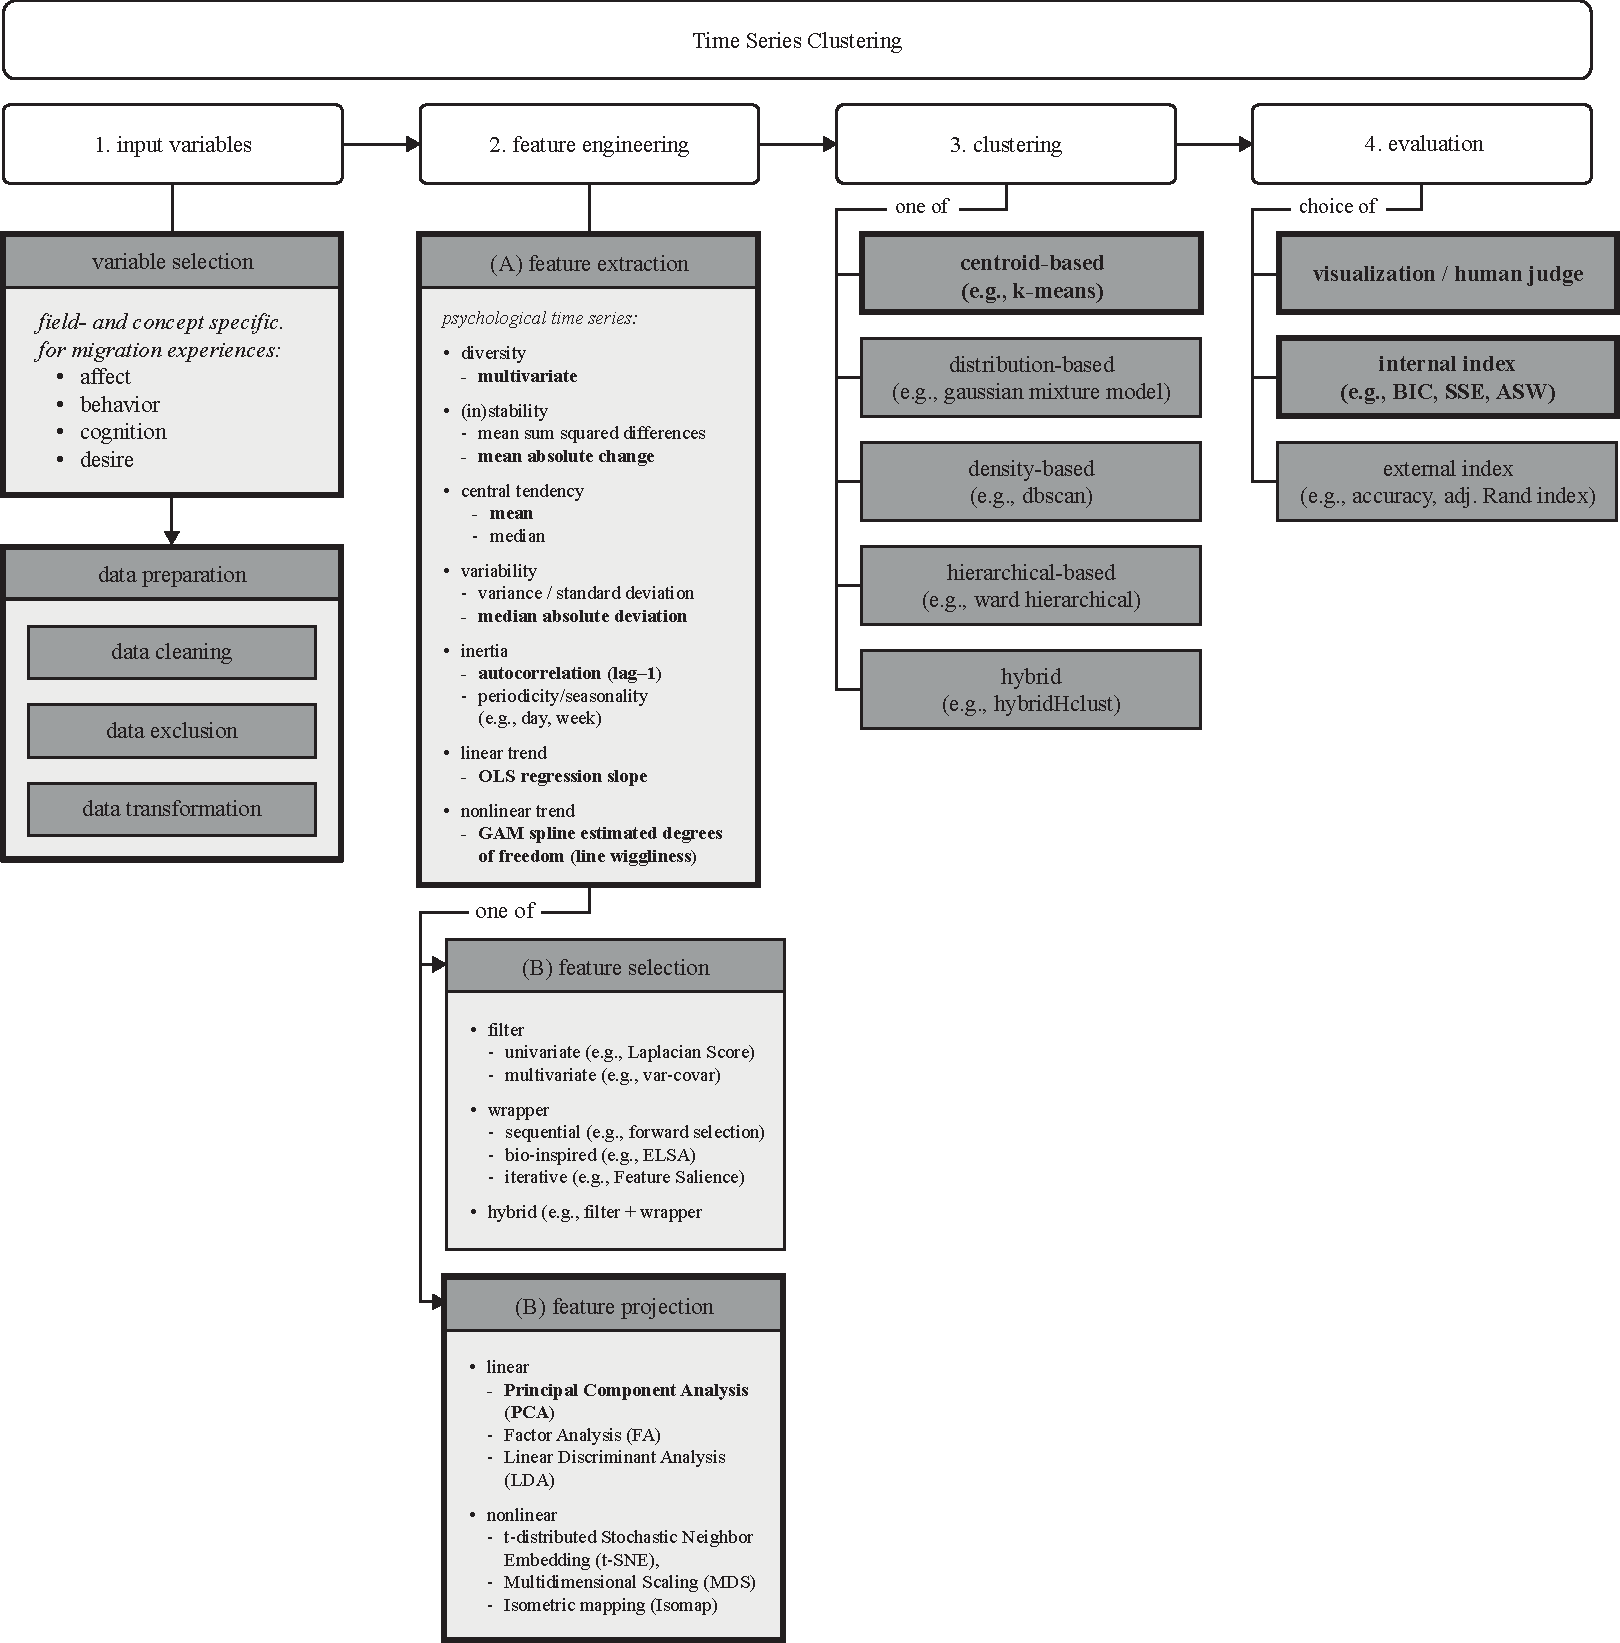
\includegraphics[width=\textwidth]{figures/TS Cluster Flow/TimeSeriesClusterFlowSelection.pdf}
  \caption*{Note: \\
  Choices selected for illustration in this manuscript are marked in bold.}
\end{figure}

\subsection{Input Variables}
Time series clustering starts with the selection and preparation of the variables of interest. While the selection will necessarily be field- and concept-specific, there are a few conceptual and methodological issues that should be considered. Conceptually, the included variables should adequately capture the concept of interest and should be meaningful to the understanding of the time series. One of the advantages of feature-based clustering is that it is inherently adept to accomodating multi-variate concepts --- a common aim in ESM research. There are, for example, calls that emotion dynamics should be assessed with a repertoire of positive and negative emotions \citep[e.g.,][]{dejonckheere2019}, many health developments are captured within the biopsychosocial domains \citep[e.g.,][]{suls2004}, and migration experiences are fully captured with affect, behavior, cognition, and desire measurements \citep[e.g.,][]{Kreienkamp2022d}. At the same time, however, the added number of variables can become a methodological concern. Not only can redundant and irrelevant variables diminish the quality of the analyses, but with intensive longitudinal data the number of data points compounds across participants, measurement occasions, and variables so that additional variables can make many of the following steps substantially more difficult (also see \fgrref{fig:TSCFlowN}). 

\begin{figure}[!ht] %hbtp
  \caption{Exemplary Flowchart of Data Points in Feature-Based Time Series Clustering}
  \label{fig:TSCFlowN}
  \centering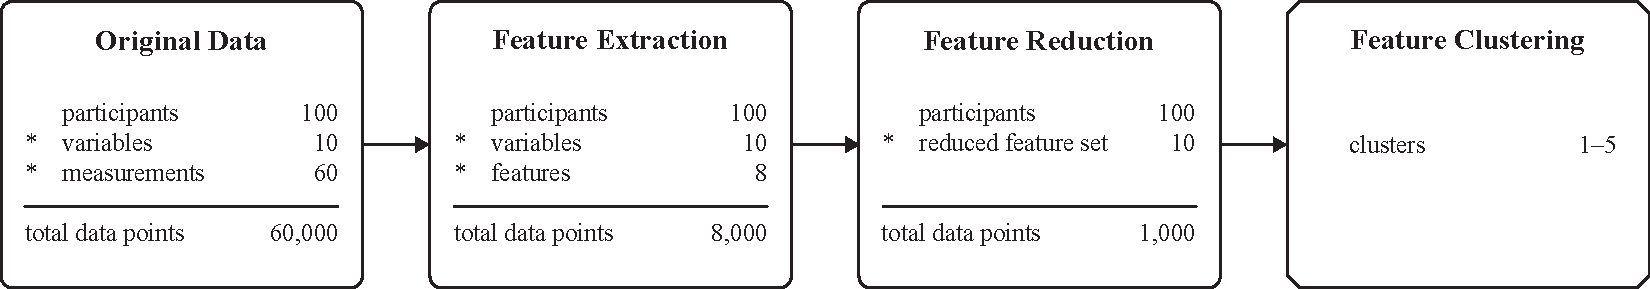
\includegraphics[width=\textwidth]{figures/TS Cluster Flow/tsClustFlowN.pdf}
  \caption*{Note: \\
  The presented number of participants, variables, and measurement occasions are somewhat arbitrary but generally represent common sample sizes found within the literature. Also the number of extracted clusters is presented for illustrative purposes only.}
\end{figure}

For our illustration, we include 12 variables that were available across
all three studies and captured information about the participant's
interactions, as well as cognitive-, emotional-, and motivational self
in relationship with the majority group. We chose these aspects in
particular because (1) the interaction-specific information exemplified
the structural missingness issue of modern ESM data and (2) the
motivational, emotional, and cognitive experience offered a diverse
conceptualization of migration experience (beyond behavioral
measurements) that is becoming more common in the literature
\citep[][]{Kreienkamp2022d}. Full methodological details are available
in Online Supplemental Material A, but basic item information,
descriptives, and correlations are also available in
\tblref{tab:descrLong}.

Once the important variables have been selected, the data needs to be
prepared for the analysis steps. Importantly, this not only means
validating and cleaning the data (e.g., re-coding, removing duplicate or
unwanted measurements) but also making the time series comparable. Two
important steps are making the time-frames and response scales
comparable across participants --- for example, by choosing a time frame
that is common to most participants and standardizing the participants'
responses \citep{liao2005}.

In our illustration data set, the studies differed substantially in the
maximum length of participation (\(\text{max}(t_{S1})=\) 63,
\(\text{max}(t_{S2})=\) 69, \(\text{max}(t_{S3})=\) 155). This was
likely due to the option to continue participation without compensation
in the later two studies. To make the three studies comparable in
participation and time frames, we iteratively removed all measurement
occasions and participants that had more than 45\% missingness
\citep[which was in line with the general rcecommendation for data that might still need to rely on imputations for later model testing][]{Madley-Dowd2019}.
This procedure let to a final sample of 157 participants, who jointly
produced 8,132 measurements. Importantly, both the participant
repsonse-patterns and the time frame were now substantially more
comparable (\(\text{max}(t_{S1})=\) 61, \(\text{max}(t_{S2})=\) 60,
\(\text{max}(t_{S3})=\) 67). For a full overview of the data reduction
procedure and study-specific exclusions see Online Supplemental Material
A.

\begin{sidewaystable*}[!hbtp]
\centering

\caption{\label{tab:descrLong}Correlation Table and Descriptive Statistics}
\centering
\resizebox{\linewidth}{!}{
\begin{tabular}[t]{lcccccccccccc}
\toprule
  & \makecell{Int: \\ Accidental} & \makecell{Int: \\ Voluntary} & \makecell{Int: \\ Cooperative} & \makecell{Int: \\ Representative} & \makecell{Int: \\ Meaningful} & \makecell{Int: \\ Quality} & Core Need & \makecell{Core Need \\ Due to Partner} & \makecell{Attitude \\ Partner} & \makecell{Daytime \\ Core Need} & \makecell{Outgroup \\ Attitude} & Well-being\\
\midrule
\addlinespace[0.3em]
\multicolumn{13}{l}{\textbf{Correlations}}\\
\hspace{1em}Int: Accidental &  & -0.20 & -0.21* & 0.07 & -0.10 & -0.13 & -0.39*** & -0.26* & -0.05 & -0.28** & -0.03 & 0.12\\
\hspace{1em}Int: Voluntary & -0.14*** &  & 0.63*** & -0.04 & 0.12 & 0.44*** & 0.19 & 0.16 & 0.42*** & 0.10 & 0.25** & -0.05\\
\hspace{1em}Int: Cooperative & -0.14*** & 0.32*** &  & 0.19 & 0.38*** & 0.68*** & 0.42*** & 0.53*** & 0.47*** & 0.24* & 0.28** & -0.08\\
\hspace{1em}Int: Representative & 0.28*** & 0.39*** & -0.11*** &  & 0.10 & 0.13 & -0.09 & -0.03 & 0.14 & -0.02 & 0.43*** & -0.07\\
\hspace{1em}Int: Meaningful & 0.01 & 0.06** & 0.21*** & 0.30*** &  & 0.66*** & 0.11 & 0.20 & 0.44*** & 0.10 & 0.01 & -0.03\\
\hspace{1em}Int: Quality & 0.07** & 0.44*** & 0.33*** & 0.04 & 0.16*** &  & 0.42*** & 0.34*** & 0.65*** & 0.23* & 0.25* & 0.07\\
\hspace{1em}Core Need & 0.12*** & -0.07** & 0.08*** & 0.41*** & 0.02 & -0.02 &  & 0.65*** & 0.11 & 0.64*** & 0.15 & 0.30**\\
\hspace{1em}Core Need Due to Partner & -0.18*** & 0.18*** & 0.20*** & 0.58*** & 0.15*** & 0.15*** & 0.19*** &  & 0.14 & 0.53*** & 0.13 & 0.07\\
\hspace{1em}Attitude Partner & 0.21*** & 0.27*** & 0.32*** & 0.24*** & 0.17*** & 0.17*** & 0.22*** & 0.16*** &  & -0.09 & 0.57*** & 0.08\\
\hspace{1em}Daytime Core Need & 0.29*** & 0.10*** & 0.53*** & 0.26*** & 0.15*** & 0.14*** & 0.37*** & 0.17*** & 0.33*** &  & 0.07 & 0.17\\
\hspace{1em}Outgroup Attitude & 0.01 & 0.18*** & -0.04 & -0.06* & 0.14*** & 0.20*** & 0.09*** & -0.03 & 0.16*** & 0.26*** &  & 0.21*\\
\hspace{1em}Well-being & -0.09*** & 0.33*** & 0.30*** & 0.11*** & 0.09*** & 0.31*** & -0.06** & 0.23*** & 0.14*** & 0.20*** & 0.24*** & \\
\addlinespace[0.3em]
\multicolumn{13}{l}{\textbf{Descriptives}}\\
\hspace{1em}Grand Mean & 39.10 & 80.08 & 79.55 & 64.65 & 61.16 & 79.85 & 85.42 & 78.52 & 80.59 & 76.48 & 66.84 & 49.64\\
\hspace{1em}Between SD & 31.14 & 20.61 & 18.41 & 21.12 & 24.62 & 17.05 & 16.01 & 21.53 & 16.33 & 21.63 & 18.54 & 31.95\\
\hspace{1em}Within SD & 28.72 & 19.27 & 17.43 & 19.92 & 22.32 & 16.37 & 18.63 & 20.02 & 15.81 & 22.26 & 9.45 & 25.72\\
\hspace{1em}ICC(1) & 0.21 & 0.29 & 0.27 & 0.35 & 0.31 & 0.25 & 0.18 & 0.26 & 0.25 & 0.20 & 0.77 & 0.52\\
\hspace{1em}ICC(2) & 0.90 & 0.93 & 0.93 & 0.89 & 0.94 & 0.92 & 0.91 & 0.92 & 0.91 & 0.92 & 0.99 & 0.98\\
\bottomrule
\multicolumn{13}{l}{\rule{0pt}{1em}\textit{Note: }}\\
\multicolumn{13}{l}{\rule{0pt}{1em}Upper triangle: Between-person correlations;}\\
\multicolumn{13}{l}{\rule{0pt}{1em}Lower triangle: Within-person correlations;}\\
\multicolumn{13}{l}{\rule{0pt}{1em}*** p < .001, ** p < .01,  * p < .05}\\
\end{tabular}}
\end{sidewaystable*}



\subsection{Feature Extraction}
Armed with a relevant selection of key variables, the main aim of the feature extraction is to describe the most important and meaningful aspects of a time series. In its most general approach, feature extraction can include any numeric summary of the time series \citep[e.g.,][]{maharaj2019}. Given this flexibility, a staggering variety of time series features have been proposed across different disciplines. For example, \citet{wang2006} proposed 9 structural characteristics \citep[also see][]{fulcher2013}, \citet{adya2001} collected 28 features relevant for forecasting, and a commonly used software package for feature extraction `tsfresh' allows users to extract a total of 794 features of a time series \citep[][]{christ2018}. 

However, not all time series features might be relevant to psychological time series or any particular research question. For example, a psychologist interested in well-being might not necessarily be interested in the exact time point after which 50\% of the summed well-being values lie (i.e., relative mass quantile index) or how much different sine wave patterns within the well-being data correlate with one another (i.e., cross power spectral density). Instead, we advocate that we look at time series features that have a strong backing within the ESM literature and offer meaningful interpretability. 

Fortunately, past conceptual and empirical efforts offer valuable discussions of common time series features in psychological research. To understand emotion dynamics, \citet{kuppens2017} originally proposed four features: (1) within-person variability, (2) co-variance or ICC, (3) inertia or autocorrelation, and (4) cross-lagged correlations. These features were then extended by \citet{krone2018}, adding (5) innovation variance, and (6) mean intensity. \citet{krone2018} even built a parametric model to tentatively cluster study participants. From a slightly different perspective \citet{dejonckheere2019} later added three additional features for psychological time series: (7) instability (8) interdependence (i.e., network density), and (9) diversity \citep[i.e., Gini coefficient; also see][]{wendt2020}\footnote{It should be noted that also within the psychological literature, alternative summaries have been proposed that, for example, include measurement distribution, nonlinear developments, or categorical states. As an example, \citet{kiwuwa-muyingo2011} proposed to extract clinically meaningful states for medical adherence data and suggests these states as meaningful time series features.}. 

Some of the features found in the psychological literature are not necessarily well-suited to summarize time series for feature-based clustering and some key conceptual features are not well represented in the literature. In particular, covariances and cross-lagged correlations often produce a large number of parameters and might not necessarily summarize the existing data enough \citep{ernst2021}. Others such as network density parameters, used to summarize variable interdependence, might not always be meaningful for psychological data \citep{bringmann2019a}. At the same time, linear and nonlinear trends are not captured by the features commonly proposed for psychological time series, because the features are often developed for stationary models \citep[e.g.,][]{krone2018}. 

Thus, while the final selection of features should always be driven by the research questions and field-specific conventions, for our illustration we chose six features that relate to common psychological research questions and recent works within the field: (1) central tendency, (2) variability, (3) instability, (4) self-similarity, (5) linear trend, and (6) nonlinearity. An overview of the selected features, their substantive interpretations, and mathematical operationalizations is also available in \tblref{tab:esmFeatures}. We provide additional background on the theoretical relevance of the selected features in \appref{app:FeatureBackground}. For each of the six time series features we chose, we chose a mathematical representation that was appropriate for our type of data. We provide a short introduction of each feature below. Beyond the operationalizations we chose for our case study, we provide an R-function that automatically extracts and prepares a large selection of the time series feature operationalizations presented in \tblref{tab:esmFeatures} in our GitHub repository (see the \texttt{featureExtractor} function).

%\begin{table}%[hbt]
\begin{sidewaystable*}[!hbtp]
    \centering
    \caption{Examples of Features for Psychological Time Series.}
    \label{tab:esmFeatures} 
    \begin{tabular}{
    >{\raggedright\arraybackslash}p{0.15\linewidth} 
    >{\raggedright\arraybackslash}p{0.35\linewidth} 
    >{\raggedright\arraybackslash}p{0.25\linewidth} 
    >{\raggedright\arraybackslash}p{0.20\linewidth}
    }
        \hline 
        Time Series Feature & Substantive Interpretation & Example Operationalizations & Formulas, refs, ...? \\ 
        \hline \\ [-0.5em]
        
        %Diversity \newline \hl{(drop this \& keep in var. selection only?)} & 
        %Multivariate measurement of concepts (e.g., affect-behavior-cognition-desire, or bio-psycho-social) \linebreak & 
        %-----\linebreak  & 
        %{\centering --- ? ---\par} \\
        
        Central Tendency \linebreak & 
        Average level of the experience across the entire measurement period. \linebreak & 
        \vspace{-1em}
        \begin{itemize}[nosep,leftmargin=*,label={--}]
            \item mean
            \item median
            \item mode
        \end{itemize} \linebreak  & 
        {\centering --- ? ---\par} \\ 
        
        Variability & 
        Describes the average deviation from the central tendency across the entire measurement period. \linebreak & 
        \vspace{-1em}
        \begin{itemize}[nosep,leftmargin=*,label={--}]
            \item standard deviation
            \item variation coefficient
            \item median absolute deviation
        \end{itemize} \linebreak & 
        {\centering --- ? ---\par} \\ 
        
        (In)stability & 
        Describes the average change between two consecutive measurements of the experience. \linebreak & 
        \vspace{-1em}
        \begin{itemize}[nosep,leftmargin=*,label={--}]
            \item mean sum squared differences
            \item mean absolute change
            \item Ix instability index
        \end{itemize} \linebreak & 
        {\centering --- ? ---\par} \\ 
        
        Inertia & 
        Describes how much experiences carry over to the future measurements. This includes resistance to change (i.e., carries over to the next measurement) and periodic or seasonal returns (e.g., self-predictive on a daily or weekly basis). \linebreak &
        \vspace{-1em}
        \begin{itemize}[nosep,leftmargin=*,label={--}]
            \item autocorrelation (e.g., lag–1)
            \item fourier coefficients
            \item continuous wavelet transform
        \end{itemize} \linebreak & 
        {\centering --- ? ---\par} \\ 

        Linear Trend & 
        Describes upwards or downwards linear trend of the experience reports. \linebreak & 
        \vspace{-1em}
        \begin{itemize}[nosep,leftmargin=*,label={--}]
            \item OLS regression slope
            \item avg. piecewise linear reg. slope
        \end{itemize} \linebreak & 
        {\centering --- ? ---\par} \\ 
        
        Nonlinearity & 
        Describes the nonlinear structure of the time series. This includes measures that indicate the deviation from the a linear trend as well as nonlinear model parameters. \linebreak & 
        \vspace{-1em}
        \begin{itemize}[nosep,leftmargin=*,label={--}]
            \item GAM spline edf
            \item bicoherence metrics
            \item Langevin polinomial coefficient
        \end{itemize} \linebreak & 
        {\centering --- ? ---\par} \\ 
        
        \hline \\ [-0.75em]
        \multicolumn{4}{p{\linewidth}}{\footnotesize \textit{Note.} The presented features and operationalizations are neither exhaustive nor necessary for feature-based clustering.}
    \end{tabular}
\end{sidewaystable*}


\paragraph{Central tendency.}

The central tendency refers to the statistical measures that represent
the ``typical'' or ``average'' of a set of data. The most common
measures of central tendency are the mean, median, and mode
\citep{weisberg1992}. As a familiar statistic from probability theory,
the central tendency sits at the heart of many fundamental questions
about psychological time series. Researchers might, for example, be
interested in whether ``Over a one-month period, are some people happier
than others?''

For the central tendency feature of our illustration we chose the robust
\textit{median}, which can avoid potential issues with non-normally
distributed time series responses or outliers \citep{weisberg1992}. To
calculate the \textit{median} (\(M\)), we let \(X_{ij}\) be the ordered
list of values from the time series of variable \(j\) for participant
\(i\). The calculation depends on whether the number of measurements in
a time series \(n\) is odd or even.

\begin{equation} \label{eq:median}
  M(X_{ij}) = 
    \begin{cases}
      X \left[ \frac{n+1}{2} \right] & \text{if $n$ is odd} \\
      \frac{X \left[ \frac{n}{2} \right] + X \left[ \frac{n}{2} +1 \right]}{2} & \text{if $n$ is even}
    \end{cases}
\end{equation}

\paragraph{Variability.}

Variability captures the degree to which a set of data differs from the
central tendency and is sometimes also referred to as the dispersion or
spread of the data \citep{weisberg1992}. In time series analyses,
variability is conceptually important because information about the
distribution and diversity of the data has been found to be indicative
of worse psychological states \citep{myin-germeys2018, helmich2021}.
Person-level differences of ESM measurements have, for example, been
associated with higher levels of psycho-pathological recurrences among
depression patients \citep{timm2017}. As such, psychological researchers
and practitioners are often empirically interested in between-person
differences in variability. Researchers on polarization and
radicalization might for example ask: ``Are people settled in their
attitudes towards migrants or do they vary across the measurement
period?''

For our illustration data, we chose to capture the time series
variability with the \textit{Median Absolute Deviation} (\(MAD\)), where
we calculate the \textit{median} (\(M\); calculated as in
\equatref{eq:median}) for the absolute deviations of measurement \(x\)
at time point \(t\) for participant \(i\) and variable \(j\) from the
median of that time series \(X\). We again chose the robust statistic
because the Median-based measure is less affected by non-normal
distributions and extreme values or outliers compared to other measures
of variability like the standard deviation \citep{weisberg1992}

\begin{equation} \label{eq:mad}
  MAD(X_{ij}) = M(\left| x_{ijt} - M(X_{ij}) \right|)
\end{equation}

\paragraph{Instability.}

Instability captures the average change between two consecutive
measurements \citep{ebner-priemer2009}. While instability is
conceptually related to the variability feature, variability does not
take into account temporal dependency, whereas instability looks at the
`jumpy-ness' of the data over time. In other words, variability reflects
the range or diversity of values in a time series data, while
instability reflects the fluctuation or inconsistency in a time series
data over time \citep{trull2008}. For example, if a person has rapid and
extreme changes in mood their mood is highly unstable, while if a
person's mood responses span a wide range over the entire study period,
their mood is highly variable \citep{jahng2008}. Within psychological
time series, instability measurements have especially been important in
the research of borderline personality disorder \citep{trull2008} and
suicidality \citep{kivela2022}, but also in understanding early warning
signals more generally \citep{wichers2019}. Conceptually, the
instability feature, thus, relates to a broad range of research
questions, including: ``What is the nature of the identification changes
in those who start working in a new country?'' or ``Do strong daily
fluctuations in self-esteem reflect the process of identity formation in
adolescents?''

For our data we chose the \textit{mean absolute change}
\citep[$MAC$; e.g.,][]{ebner-priemer2009, barandas2020}, which looks at
the average absolute difference of two consecutive measurements \(x\) at
time points \(t\) and \(t-1\), for each time series \(X\) of participant
\(i\) and variable \(j\).

\begin{equation} \label{eq:mac}
  MAC(X_{ij}) = \frac{1}{n-1} \sum_{t=2, \ldots, t}\left|x_{t}-x_{t-1}\right|
\end{equation}

Another common measurement of instability is the
\textit{Mean of the Squared Successive Differences} (\(MSSD\)), which is
often preferred where differences in magnitude are more important than
the frequency of those changes, for example, when big shifts in time
series are considered more impactful or when outliers are meaningful and
need to be taken into account \citep{chatfield2003}.

\paragraph{Self-similarity.}

Self-similarity in time series data refers to the property of a time
series to exhibit similar patterns of behavior over different time
scales \citep{dmello2021}. That is, self-similarity describes how much a
measurement carries over to future measurements. One important
self-similarity in psychological time series is \texit{inertia} --- how
much a measurement carries over to its next measurement
\citep{kuppens2010, suls1998}. If inertia is high a development tends to
stay in a certain state. Because high inertia is resistant to change, in
emotion dynamics high inertia of negative affect has been found to be
indicative of under-reactive systems and to be characteristic of
psychological maladjustment \citep{kuppens2010}. In a similar vein, high
inertia in negative affect at baseline was even predictive of the
initial onset of depression \citep{kuppens2012}. Conceptually, inertia
is more broadly connected to research questions such as:
\texttt{Do\ patients\ stay\ in\ a\ negative\ mood\ for\ several\ measurements?\textquotesingle{}\textquotesingle{}\ or}Do
migrants stay with their language practice for several days at a
time?'\,'

For our illustration case, we chose the commonly used autocorrelation or
autoregression with a lag-1 to capture the inertia. High autocorrelation
values can indicate high levels of inertia, while low autocorrelation
values may indicate a more unpredictable or volatile time series
\citep{dejonckheere2019}. The lag--1 autocorrelation \(r_{ij,1}\) looks
at the average correlation between a measurement \(x\) and the preceding
measurement \(x_{t-1}\) for the time series \(X\) of participant \(i\)
and variable \(j\) with \(n\) measurements.

\begin{equation} \label{eq:ar}
  r_{ij,1} = \frac{\sum_{t=2}^{n}(x_{ijt}-\overline{x}_{ij})(x_{ij,t-1}-\overline{x}_{ij})}{\sum_{t=1}^{n}(x_{ijt}-\overline{x}_{ij})^2}
\end{equation}

Where \(\overline{x}_{ij}\) is the mean of the time series \(x_{ij}\),
calculated as:

\begin{equation} \label{eq:mean_for_ar1}
  \overline{x}_{ij} = \frac{1}{n} \sum_{t=1}^{n} x_{ijt}
\end{equation}

\paragraph{Linear trend.}

In non-stationary time series, a linear trend can be observed when there
is a consistent increase or decrease in the data over time
\citep{nyblom1986}. For psychological time series, researchers have, for
example, pointed out the importance of linear trends in interpersonal
communications \citep{vasileiadou2014}, and emotion dynamics
\citep{oravecz2016}. Theoretically, linear trends are often considered
the simplest way of assessing whether a psychological theory of change
is appropriate \citep{gottman1969}. In empirical practice, linear trends
are, thus, commonly exemplified by research questions such as ``Do
patient symptoms improve consistently?'' or ``Does worker productivity
decline continuously?''

For the variables in our illustration data set, we chose an overall
linear regression slope to capture the linear trend. The regression
slope \(b_{ij}\) provides the average change from one time point \(t\)
to the next across all measurements \(x\) of a time series \(X\) of
participant \(i\) and variable \(j\). The specific form of the OLS slope
formula we provide below calculates \(b_{ij}\) as the sum across all
time points of the product of the deviation of time \(t\) from its mean
\(\overline{t}\) and the deviation of \(x_{ij}\) from its mean
\(\overline{x}_{ij}\) at each time point, divided by the sum across all
time points of the square of the deviation of time from its mean
(\(\sum(t-\overline{t})^2\)). Intuitively, the formula captures the rate
of change of variable \(x_{ij}\) with respect to time. This slope will
indicate how the variable \(x_{ij}\) changes over time, controlling for
its mean value and the mean of time. If the slope is positive,
\(x_{ij}\) increases over time; if it's negative, \(x_{ij}\) decreases
over time.

\begin{equation} \label{eq:lin}
  b_{ij} = \frac{\sum(t-\overline{t})(x_{ijt}-\overline{x}_{ij})}{\sum(t-\overline{t})^2}
\end{equation}

\paragraph{Nonlinearity.}

Changes in psychology are not always linear, instead, nonlinearity is a
common feature of psychological time series \citep{hayes2007}. As an
example, episodic disorders, such as depression, are most likely best
described as non-linear systems \citep{hosenfeld2015}. Similarly,
patients in recovery from depression showed sudden changes in the
improvement of depression \citep{helmich2020a}. But also substance abuse
\citep{boker1998} or attitude changes rarely develop linearly
\citep{vandermaas2003}. Conceptually, researchers might have research
questions about the type of the development: ``Is the development of
well-being a nonlinear process?'' as well as the shape and structure of
the development: ``How many spikes in well-being did a migrant
experience?''

We summarized the nonlinear trend with the
\textit{estimated degrees of freedom} of an empty GAM spline model. The
\(edf\) summarizes the \textit{wiggliness} of a spline trend line
\citep{wood2017}. The degrees of freedom of a spline model are primarily
determined by the number of knots and the order of the spline. For
instance, a cubic spline with \(k\) knots has \(k\)+3 degrees of freedom
\citep{faraway2016}. However, in a penalized spline framework, which is
commonly used for GAMs, the effective degrees of freedom can be less
than \(k\)+3. This is because the model employs a smoothing parameter to
control the trade-off between the complexity (flexibility) of the model
and its fit to the data, thereby penalizing overly complex models and
potentially reducing the effective degrees of freedom \citep{marx1998}.
Intuitively then an edf of 1 would be equivalent to a linear
relationship (i.e., one linear slope parameter), whereas a higher edf
(particularly an edf \textgreater{} 2) is indicative of a non-linear
trend. The estimated degrees of freedom are commonly based on a concept
called `effective degrees of freedom' and can be represented as the
trace \(tr\) (i.e., the sum of the diagonal elements) of the smoother
matrix \(S\), a symmetric matrix that maps from the raw data to the
smooth estimates \citep{wood2017}.

\begin{equation} \label{eq:df}
  edf = tr(S)
\end{equation}

Beyond our main features of interest, we also extracted the
participant's number of completed ESM measurements to ensure that the
clusters are comparable in that regard (i.e., to exclude spurious
explanations for the cluster assignments). After the feature extraction,
we found that about 1.40\% of the extracted features are missing across
the 72 features per participant. This might, for example, happen if
participants do not have two subsequent measurements with outgroup
interactions, so that an autocorrelation with lag-1 cannot be calculated
for the contact-specific variables. The small number of missing values
indicates that the feature-based approach indeed largely avoids the
structural missingness issue. However, even the few missing values can
be an issue for some feature reduction or feature clustering algorithms.
We, thus, impute the missing feature values with a single predictive
mean matching imputation using the MICE library \citep[][]{buuren2011}.
Note again that with this procedure we only need to impute an extremely
small number of missing values as most feature calculations can use the
available data instead.


It is important to reiterate that the six selected time-series features are in no way exhaustive or imperative. Both using a more data-driven approach to the selection of features or selecting entirely different aspects to summarize the time series are legitimate options \citep[e.g., see][]{heylen2016}. Our choice seeks to offer a practical toolbox of features that are common and meaningful to psychological research questions and -practice but are also easy to extract and summarize a broad range of developments without asserting strict assumptions.

\subsection{Feature Reduction}
Once a meaningful selection of time series features has been extracted for each variable and participant, the total number of data points sometimes remains too large for the desired clustering algorithm. As an example, a relatively common scenario would include 10 variables of interest, where eight time series features are extracted, resulting in 80 features per participant (with a common sample size of 100 participants that would result in a total of 8,000 data points in this hypothetical example). We offer an illustration of the compounding numbers of data points in \fgrref{fig:TSCFlowN}. The difficulty of working with such a large number of dimensions is sometimes termed the `dimensionality curse' \citep[e.g.,][]{altman2018}. To deal with this dimensionality issue, two main approaches have been proposed --- feature selection and feature projection \citep[e.g.,][also see \tblref{tab:featureReduction} for a full overview of the approaches, methods, and common algorithms]{erdogmus2008}. 

Feature selections seek to create a subset of the most important features. The many available approaches differ in how they seek to determine the importance of the individual features \citep{alelyani2014}. Generally speaking, selection methods can be categorized as `filter', `wrapper', or `hybrid' methods \citep{hoque2014}. The filter methods, broadly speaking determine important features by identifying irrelevant features (e.g., because features do not capture much information), and identifying redundant features \citep[e.g., because features capture the same information; e.g., see][]{yu2004}. Wrapper methods, on the other hand, avoid the feature-based evaluation and focus on the performance of the later model to identify the most important features \citep{kohavi1997}. A wrapper, thus, compares the performance of models with different feature combinations \citep[e.g., see][]{tang2014}. Traditional examples of wrappers are forward selection or backward elimination procedures. Because filter methods might not always perform well and wrapper methods are computationally intensive\footnote{Computationally \textit{k} features could be considered in \(2^k – 1\) possible combinations --- for the example of 80 features that would allow for \(1.20 \times 10^{24}\) (over one septillion) combinations.}, hybrid methods seek to combine the two methods and find a balance between computational effort (i.e., efficiency) and performance \citep[i.e., effectiveness; e.g.,][]{alelyani2014}. Methods might, for example, use a filter step to reduce the size of features considered in a later wrapper step \citep{hsu2011}. Feature selection procedures have the benefit that they retain the interpretable feature labels directly and immediately indicate which features were most informative in the sample.

The second general approach to the dimensionality curse has been feature projection. Broadly speaking, projection methods seek to transform the many features in such a way that a much smaller number of new variables can accurately capture the variance and structure of the original features \citep[i.e., the data is projected to a lower dimensional space; e.g.,][]{carreira-perpinan1997}. Projection methods are relatively common in psychological research --- including, factor- and principal component analyses \citep{vandermaaten2009}. Commonly, this is achieved using linear transformations \citep[e.g., principal component analysis; see][]{cunningham2015}, or more complex nonlinear transformations \citep[e.g., t-SNE; see]{lee2007}. Feature projection methods have been popular because of their widespread availability as well as their high efficiency.

%\begin{table}%[hbt]
\begin{sidewaystable*}[!hbtp]
    \centering
    \caption{Examples of Feature Reduction Approaches and Methods.}
    \label{tab:featureReduction} 
    \begin{tabular}{
    >{\raggedright\arraybackslash}p{0.08\linewidth} 
    >{\raggedright\arraybackslash}p{0.08\linewidth} 
    >{\raggedright\arraybackslash}p{0.54\linewidth} 
    >{\raggedright\arraybackslash}p{0.25\linewidth}
    }
        \hline 
        Approach & Method & Intuitive Description & Algorithm Examples \\ 
        \hline \\ [-0.5em]
        
        Selection \linebreak & 
        filter \linebreak & 
        Features are selected individually or jointly based on selection criteria. One common selection criterion is the amount of information and (unique) variance a feature captures. Univariate methodologies are able to identify irrelevant features (i.e., because features do not capture much information), multivariate methods additionally allow to remove redundant features \citep[i.e., because features capture the same information][]{yu2004}. \linebreak &
        \vspace{-1em}
        \begin{itemize}[nosep,leftmargin=*,label={--}]
            \item univariate filter (e.g., Laplacian Score)
            \item multivariate filter (e.g., variance-covariance)
        \end{itemize}
         \linebreak \\ 
        
        \linebreak & 
        Wrapper \linebreak & 
        Wrapper methodologies run models with different feature combinations and compare performance. Because the selection process is essentially a search problem this method is computationally intensive. Traditionally wrappers have used forward selections or backward eliminations but recently alternative approaches have been proposed based such as ant colony and swarm intelligence paradigms \citep[e.g., see][]{tang2014}. \linebreak &
        \vspace{-1em}
        \begin{itemize}[nosep,leftmargin=*,label={--}]
            \item sequential (e.g., forward selection)
            \item bio-inspired (e.g., ELSA)
            \item iterative (e.g., feature salience)
        \end{itemize}
         \linebreak \\ 
        
        \linebreak & 
        hybrid \linebreak & 
        Hybrid selection methodologies combine filter and wrapper methodologies to avoid the shortcomings of the individual methods. An initial filter step selects candidate features (efficiency) and a subsequent wrapper ensures high performance \citep[effectiveness; e.g.,][]{alelyani2014}. \linebreak &
        \vspace{-1em}
        \begin{itemize}[nosep,leftmargin=*,label={--}]
            \item filter + wrapper (e.g., Calinski-Harabasz Index)
        \end{itemize}
        \linebreak \\

        Projection \linebreak & 
        linear \linebreak & 
        Linear dimensionality reduction methodologies use linear transformations of the original data to stretch and shift the data in such a way that the data can be `projected' to a lower dimensional space without loosing too much information. These methods are well-established, tend to be fast, and usually do not need much conceptual input from the user \citep[][]{cunningham2015}. \linebreak &
        \vspace{-1em}
        \begin{itemize}[nosep,leftmargin=*,label={--}]
            \item Principal Component Analysis (PCA)
            \item Factor Analysis (FA)
            \item Linear Discriminant Analysis (LDA)
        \end{itemize}
         \linebreak \\
        
        \linebreak & 
        nonlinear \linebreak & 
        Nonlinear dimensionality reduction methods also seek to map high-dimensional data to a lower dimensional space. However, nonlinear methods have been developed to preserve the local and global structure of more complex multidimensional patterns \citep[e.g.,][]{lee2007}.
        \linebreak &
        \vspace{-1em}
        \begin{itemize}[nosep,leftmargin=*,label={--}]
            \item t-distributed Stochastic Neighbor Embedding (t-SNE)
            \item Multidimensional Scaling (MDS)
            \item Isometric mapping (Isomap)
        \end{itemize}
        \linebreak \\
        
        \hline \\ [-0.75em]
        \multicolumn{4}{p{\linewidth}}{\footnotesize \textit{Note.} The presented dimensionality reduction methods and -approaches are neither exhaustive nor necessary for feature-based clustering. Notable additional approaches are `embedded selection methods' that filter as part of the model estimation procedure (e.g., mixture models) and `network-based projection methods' that use neural networks to reduce dimensions (e.g., autoencoders).}
    \end{tabular}
\end{sidewaystable*}


For our own illustration data, we chose a feature projection method to
reduce the dimensionality of our extracted features. We particularly
chose the feature projection method for its broad applicability. We,
specifically, selected the commonly used
\textit{principal component analysis} (PCA). Some of the more
tailor-made feature selection algorithms can be more accurate in
reducing the feature dimensionality and might retain feature importance
information more directly, depending on the specific data structure.
However, PCAs have the distinct benefit that they are well-established
within the psychometric literature \citep{jolliffe2011} and can broadly
be applied to a wide variety of studies in an automatized manner
\citep{abdi2010}. As our aim is to present a general illustration that
can also be adopted across use cases, we present the workflow using a
PCA here but we encourage users to consider more specialized methods as
well.

To use the principal component analysis with our extracted time series
features, we first standardize all features across participants to
ensure that all features are weighted equally. We then enter all 72
features into the analysis. The PCA uses linear transformations in such
a way that the first component captures the most possible variance of
the original data
\citep[e.g., by finding a vector that maximizes the sum of squared distances][]{jolliffe2002, abdi2010}.
The following components will then use the same method to iteratively
explain the most of the remaining variance while also ensuring that the
components are linearly uncorrelated \citep{shlens2014}. In practice,
this meant that the PCA decomposed the 72 features into 72 principal
components but now (because of the uncorrelated linear transformations)
the first few principal components will capture a majority of the
variance. We can then decide how much information (i.e., variance) we
are willing to sacrifice for a reduced dimensionality. A common rule of
thumb is to use the principal components that jointly explain 70--90\%
of the original variance
\citep[i.e., cumulative percentage explained variance; e.g.,][]{jackson2003}.
For our illustration, we select the first 27 principal components that
explain 80\% of the variance in the original 72 features (reducing the
dimensionality by 62.50\%). For the extracted principal components we
save the 27 principal component scores for each participant (i.e., the
participants' coordinates in the reduced dimensional space; PC-scores).

We would like to comment on two practical matters when using principal
components --- the amount of dimensionality reduction and the
interpretation of the principal components. As for the expected
dimensionality reduction, given its methodology, PCAs tend to `work
better' at reducing dimensions with (highly) correlated variables
\citep[e.g.,][]{jolliffe2002}. Thus, with a set of very homogeneous
variables and features users will need fewer principal components to
explain a large amount of variance, while a more diverse set of
variables and features will tend to require more principal components to
capture the same amount of variance \citep[e.g.,][]{abdi2010}. Our 27
principal components are still a relatively high number of variables but
this is not surprising as we chose a diverse conceptualization and a
diverse set of time series features. As for interpretability, PCA allows
users to extract information on the meaning of the principal components.
In particular, because the principal components are linear combinations
of the original features, users can extract the relative importance of
each feature for the extracted principal components (i.e., the
eigenvectors). While this can be useful in understanding the variance in
the original data or help with manual feature selection, we use the PCA
purely to reduce the dimensionality for the clustering step. Instead of
relying on the principal components, we use the original features of
interest to interpret the later extracted clusters. We particularly
advocate for such an approach if all original features are considered
meaningful in understanding the time series and users would like to
retain the features for interpretation (irrespective of the features'
importance).


\subsection{Feature Clustering}
For the actual clustering of the time-series features, the main aim is to organize participants into groups so that the features of participants within a group are as similar as possible, while the features of people in different groups are as different as possible \citep{liao2005}. The crux of clustering is, thus, to have clearly defined and effective measurements of (dis)similarity. Most of the clustering algorithms used today use some form of distance measurement to optimize group assignment \citep[or similarity measurement for qualitative features; see][]{Aghabozorgi2015}. While others have produced excellent overviews of the many clustering approaches available \citep[e.g.,][]{xu2015}, the more readily available approaches suitable for most time series feature data can, broadly speaking, be categorized as based on (1) centroids, (2) distributions, (3) density, (4) hierarchies, or (5) a combination thereof \citep[see \tblref{tab:clusterApproaches} for an overview; also see][for a broader review]{jain1999}. 

There is, unfortunately, no one-size-fits-all solution to clustering and users will usually have to make an informed decision based on the structure of their data as well as an appropriate weighing of accuracy and efficiency. We provide a short intuitive explanation for common approaches, together with some of their characteristics and example algorithms in \tblref{tab:clusterApproaches}. For our own illustration, we have chosen that centroid-based k-means clustering. While k-means comes at the expense of high accuracy with more complex cluster shapes, we specifically chose k-means because it is an extremely efficient method that works well with large participant- and feature numbers without making too many restrictive assumptions about the shape of the data \citep{jain2010}. K-means is also well-established within the research community and has been readily implemented in many statistical software packages \citep{hand2005}. Additionally, many of the feature selection methods have specifically been designed for the well-established k-means algorithm \citep[e.g.,][]{boutsidis2010}. As such, the k-means offers a good starting point for many psychological researchers and the method should be generalizable across a relatively wide variety of projects.

%Each of these approaches can be a valuable clustering approach for time series feature data and users will usually have to make an informed decision based on the structure of their data as well as an appropriate weighing of accuracy and efficiency. As an example, under ideal conditions, most approaches are likely to provide a similar cluster solution \citep[e.g., for well-separated groups with little noise and few outliers; e.g., see][]{peng2022}. However, when the shapes of clusters, for example, become more complex in a multi-dimensional space, density-based or hierarchy-based approaches that allow for more bottom-up clustering are likely to be more accurate \citep[e.g.,][]{langfelder2008}. Yet, with higher numbers of participants and features, both density- and hierarchy-based approaches may perform less well and the more efficient centroid-based methods might be more effective \citep[e.g.,][]{jain2010}. Similarly, several of the proposed time series features are statics that are generated from Gaussian distributions and a distribution-based algorithm might be ideally suited to separate such distributions \citep[e.g.,][]{corduas2008}. Yet, in cases where misspecifications are costly, a method with fewer assumptions might be more advisable \citep[e.g.,][]{ankerst1999}.

%\begin{table}%[hbt]
\begin{sidewaystable*}[!hbtp]
    \centering
    \caption{Common Clustering Approaches.}
    \label{tab:clusterApproaches} 
    \begin{tabular}{
    >{\raggedright\arraybackslash}p{0.15\linewidth} 
    >{\raggedright\arraybackslash}p{0.40\linewidth} 
    >{\raggedright\arraybackslash}p{0.28\linewidth} 
    >{\raggedright\arraybackslash}p{0.12\linewidth}
    }
        \hline 
        Approach & Description & Characteristics & Examples \\ 
        \hline \\ [-0.5em]
        
        centroid-based \linebreak & 
        Chooses a pre-defined number of potential cluster centers in the feature space and assigns participants to closest center. Then, iteratively, moves the centers until a convergence criterion is met (e.g., all distances to centers minimized).
        \linebreak &
        \vspace{-1em}
        \begin{itemize}[nosep,leftmargin=*,label={--}]
            \item[\scriptsize\faPlusCircle] simple and efficient
            \item[\scriptsize\faPlusCircle] no assumptions
            \item[\scriptsize\faPlusCircle] well implemented
            \item[\scriptsize\faMinusCircle] may struggle with complex shapes
            \item[\scriptsize\faMinusCircle] sensitive to initial values and outliers
            %\item[\scriptsize\faMinusCircle] not suitable for non-convex data, relatively sensitive to the outliers, easily drawn into local optimal, the number of clusters needed to be preset, and the clustering result sensitive to the number of clusters \citep{xu2015}.
        \end{itemize}\linebreak & 
        \vspace{-1em}
        \begin{itemize}[nosep,leftmargin=*,label={--}]
            \item k-means
            %\item fuzzy c-means
            %\item CLARA
            \item PAM
        \end{itemize}\linebreak \\ 
        
        distribution-based \linebreak & 
        Assumes that the data points belong to one of several specific distributions (e.g., Gaussian distributions). Data points that fit to a distribution-based expectation are given higher probability of belonging to that distribution. We can then iteratively check with which model parameters the data points best fit within given number of distributions.
        \linebreak &
        \vspace{-1em}
        \begin{itemize}[nosep,leftmargin=*,label={--}]
            \item[\scriptsize\faPlusCircle] probabilistic
            \item[\scriptsize\faPlusCircle] well supported
            \item[\scriptsize\faMinusCircle] time intensive
            \item[\scriptsize\faMinusCircle] distribution and parameter sensitive
        \end{itemize}\linebreak & 
        \vspace{-1em}
        \begin{itemize}[nosep,leftmargin=*,label={--}]
            \item GMM
            %\item negative binomial model-based
            \item DBCLASD
        \end{itemize}\linebreak\\ 
        
        density-based \linebreak & 
        Assumes that clusters are regions where several data points are relatively close together (i.e., high density). Based on what is considered a dense region (e.g., radius of a region and minimum number of points the radius), points can be either be assigned to one of the clusters or be considered too far away from a dense region. \linebreak &
        \vspace{-1em}
        \begin{itemize}[nosep,leftmargin=*,label={--}]
            \item[\scriptsize\faPlusCircle] efficient
            \item[\scriptsize\faPlusCircle] no shape assumption
            \item[\scriptsize\faPlusCircle] do not assign outliers 
            \item[\scriptsize\faMinusCircle] may struggle with uneven densities
            \item[\scriptsize\faMinusCircle] sensitive to high dimensionality
        \end{itemize}\linebreak & 
        \vspace{-1em}
        \begin{itemize}[nosep,leftmargin=*,label={--}]
            \item DBSCAN
            \item OPTICS
        \end{itemize}\linebreak\\ 

        %graph-based \linebreak & 
        %``realized on the graph where the node is regarded as the data point and the edge is regarded as the relationship among data points'' \citep{xu2015} \linebreak &
        %\vspace{-1em}
        %\begin{itemize}[nosep,leftmargin=*,label={--}]
        %    \item[\scriptsize\faPlusCircle] efficient and accurate
        %    \item[\scriptsize\faPlusCircle] no shape assumption
        %    \item[\scriptsize\faMinusCircle] sensitive to graph complexity
        %\end{itemize}\linebreak & 
        %\vspace{-1em}
        %\begin{itemize}[nosep,leftmargin=*,label={--}]
        %    \item MST-based
        %    \item CLICK
        %\end{itemize}\linebreak\\ 

        hierarchy-based \linebreak & 
        Builds a hierarchy of cluster by step-wise combining the closest two clusters (bottom-up; agglomerative) or top down dividing the data into smaller clusters that maximize distances (top-down; divisive).
        \linebreak &
        \vspace{-1em}
        \begin{itemize}[nosep,leftmargin=*,label={--}]
            \item[\scriptsize\faPlusCircle] flexible number of clusters
            \item[\scriptsize\faPlusCircle] no shape assumption 
            \item[\scriptsize\faMinusCircle] best with small number of cases
            \item[\scriptsize\faMinusCircle] no reversal of assignments
        \end{itemize}\linebreak & 
        \vspace{-1em}
        \begin{itemize}[nosep,leftmargin=*,label={--}]
            \item Chameleon
            \item CURE
        \end{itemize}\linebreak \\ 
        
        hybrid \linebreak & 
        Usually combines different approaches, which combine the strength of the complementary approaches. Oftentimes the combination also increases efficiency. \linebreak &
        \vspace{-1em}
        \begin{itemize}[nosep,leftmargin=*,label={--}]
            \item[\scriptsize\faPlusCircle] avoids individual shortcomings
            \item[\scriptsize\faMinusCircle] less readily available
        \end{itemize}\linebreak & 
        \vspace{-1em}
        \begin{itemize}[nosep,leftmargin=*,label={--}]
            \item DD-means
            \item hybridHclust
        \end{itemize}\linebreak\\ 
        
        \hline \\ [-0.75em]
        \multicolumn{4}{p{\linewidth}}{\footnotesize \textit{Note.} The presented clustering approaches and algorithms are neither exhaustive nor necessary for feature-based clustering. Notably, recently innovations have been made based on graph-, fractal-, swarm, and quantum theory \citep[for a more in-depth review see][]{xu2015}.}
    \end{tabular}
\end{sidewaystable*}


For the actual k-means clustering, the analysis seeks to minimize the
total within-cluster variation. We used the Hartigan and Wong algorithm,
which is a widely used approach in k-means clustering of time series
features \citep{hartigan1979}. This algorithm is designed to optimize
the clustering of the feature data into \(k\) groups, where \(k\) is a
pre-defined number of clusters. The algorithm starts by randomly
separating the data points into k clusters and then iteratively updates
the assignment of each point to the nearest cluster center until
convergence. The Hartigan and Wong algorithm specifically calculates the
within-cluster variation (\(W\)) of cluster \(C_i\) as the summed
squared Euclidean distances of the feature \(x\) to its assigned cluster
centroid \(\mu_i\):

\begin{equation} \label{eq:kWCi}
  W(C_i) = \sum_{x \in C_i}(x-\mu_i)^2
\end{equation}

By summing the within cluster sum of squares from all \(k\) clusters, we
can then derive the total within-cluster sum of square \(WCSS\):

\begin{equation} \label{eq:kWCSS}
  WCSS = \sum_{i=1}^k W(C_i) = \sum_{i=1}^k \sum_{x \in C_i} (x - \mu_i)^2
\end{equation}

It is this \(WCSS\) that becomes the objective function to be minimized,
by iteratively moving features from one cluster to another
\citep{hartigan1979}. In particular, the algorithm (1) calculates the
cluster centroids of the initial partitioning, (2) checks whether any
feature has a centroid that is closer than that of the currently
assigned cluster (3) updates the centroids based on any reassigned
features, and then iterates between steps two and three until \(WCSS\)
is minimized (i.e., locally optimal convergence) or a maximum number of
iterations is reached. Given the iterative nature of the algorithm, the
initial partitioning is often important because the algorithm might
arrive at a suboptimal clustering where the \(WCSS\) cannot be further
reduced by moving any feature to another cluster, despite a better
solution existing (i.e., a local minimum). It is, therefore often
recommended to run the k-means clustering with several different
starting positions.

In our case we used the Elbow and the Silhouette method to determine the
recommended number of \(k\) clusters, which for both methods suggested
two clusters (see Supplemental Material A). We then entered the
participants' PC-scores from the previous step into the k-means
algorithm. To avoid local minima we used 100 random initial centroid
positions. In the final solution the k-means analysis assigned 80
participants to cluster 1 and 76 participants to cluster 2.


\subsection{Cluster Evaluation}
Now that the participants have been assigned to their respective clusters based on the similarity of their time series features, the final evaluation step includes two main elements, (1) evaluating the performance of the clustering analyses to choose an optimal solution and (2) interpreting the extracted clusters conceptually. 

\subsubsection{Performance}
Performance evaluation often means assessing the accuracy, stability, and separation or purity of the clustering \citep{keogh2003}. Importantly, any evaluation of the results depends on the research questions, the data, and the methods used. However, broadly speaking, evaluation methods can be categorized based on whether the true cluster labels are known or not \citep{saxena2017}. If true class labels are known, the cluster assignments can be compared to the true class labels --- using measures such as the F-measure, adjusted Rand index, mutual information, and normalized mutual information \citep[i.e., external evaluation; e.g.,][]{liao2005}. However, if the true cluster assignments are unknown, as with our psychological time series, the quality of the clusters is assessed based on the characteristics of the data itself \citep[i.e., internal evaluation; e.g.,][]{Aghabozorgi2015}. 

In our own illustration example, we used the \texttt{cluster.stats()}
function from the \texttt{fpc} \textsf{R} package, which calculates a
wide variety of internal cluster validity statistics for each of the
extracted clustering solutions. With real-world data no single
evaluation measure is likely perfect, and different measures may produce
different results depending on the characteristics of the data and the
research question being addressed \citep{kittler1998}. It is therefore
important to consider a variety of evaluation measures and to carefully
interpret the results in the context of the specific analysis
\citep{vinh2009}. We found that across most indices, the analysis with
\(k=2\) clusters performed the best. Three commonly reported indices we
would like to highlight are the comparison of within clusters sum of
squares, the average silhouette score, and the Calinski-Harabasz index.
The first statistic we looked at was the a total within-cluster sum of
square \(WCSS\) (also see \equatref{eq:kWCSS}). While the within cluster
variation will naturally decrease with (more) smaller clusters, we
observed that the decrease in \(WCSS\) was largest until \(k=2\) after
which the decrease was much smaller. This method is also called the
\textit{elbow method} \citep{syakur2018}. We then looked at a second,
commonly used measure, the average silhouette score. This statistic
measures the degree to which each time feature data point is similar to
other points within the same cluster, compared to points in other
clusters \citep{rousseeuw1987}. In our case, the \(k=2\) solution
maximized the silhouette coefficient (\(s_2=\) 0.09). Finally, the
Calinski-Harabasz index assesses the compactness and separation of the
clusters by asssessing the ratio of the sum of between-clusters
dispersion and of inter-cluster dispersion for all clusters --- thus,
the higher the score the better the performances \citep{calinski1974}.
In our case the \(k=2\) solution also showed the highest
Calinski-Harabasz index (\(CH_2=\) 16.38; a full table of all extracted
validity statistics is available in Supplemental Material
A)\footnote{It is important to note that another commonly assessed aspect of the evaluation is determining the stability and robustness of the clusters \citep{berkhin2006}. This can be assessed by evaluating the sensitivity of the clusters to different feature sets or clustering algorithms, or by using techniques such as bootstrapping to assess the uncertainty of the clusters \citep{vinh2009}. Especially when comparing different clustering algorithms one common index is the Bayesian information criterion (BIC), where a lower BIC indicates that a model is more representative of the data \citep{vandeschoot2017}.}.
In the final \(k=2\) solution the k-means analysis also assigned a
relatively even number of participants to cluster 1 (\(n_{C_1}=\) 80)
and cluster 2 (\(n_{C_1}=\) 76).


\subsubsection{Interpretation}
The interpretation of feature-based time series clustering in psychology involves understanding the meaning and implications of the obtained clusters. In order to make sense of the clustering results, we here focus on three general aspects of the results \citep{kaufman1990}. (1) Assessing differences between the clusters in the original time series features, (2) comparing the clusters based on prototype developments, (3) comparing the clusters based on between-person differences that were not included in the initial clustering.

We first inspect the clusters based on the average values of meaningful
features (see \fgrref[A]{fig:clusterFeatVar}; \citealp{Kennedy2021}). We
(1) see that for some variables the features are generally stronger in
separating the clusters (e.g., `how cooperative an interaction was'
compared to `attitudes towards the Dutch'). Additionally, we see that
(2) within the variables some features are better at distinguishing
clusters (e.g., median of well-being vs.~MAC of well-being). We then
inspect the clusters with a focus on the features (see
\fgrref[B]{fig:clusterFeatVar}). While this is the same data as for the
variable focus, we can see more clearly that some features are better at
distinguishing the clusters across variables (e.g., mean and median
compared to auto correlations). This offers some information on which
features were are most important in understanding the two extracted
groups.

\begin{figure}[!ht] %hbtp
  \caption{Cluster Group Comparisons based on Features and Variables}
  \label{fig:clusterFeatVar}
  \centering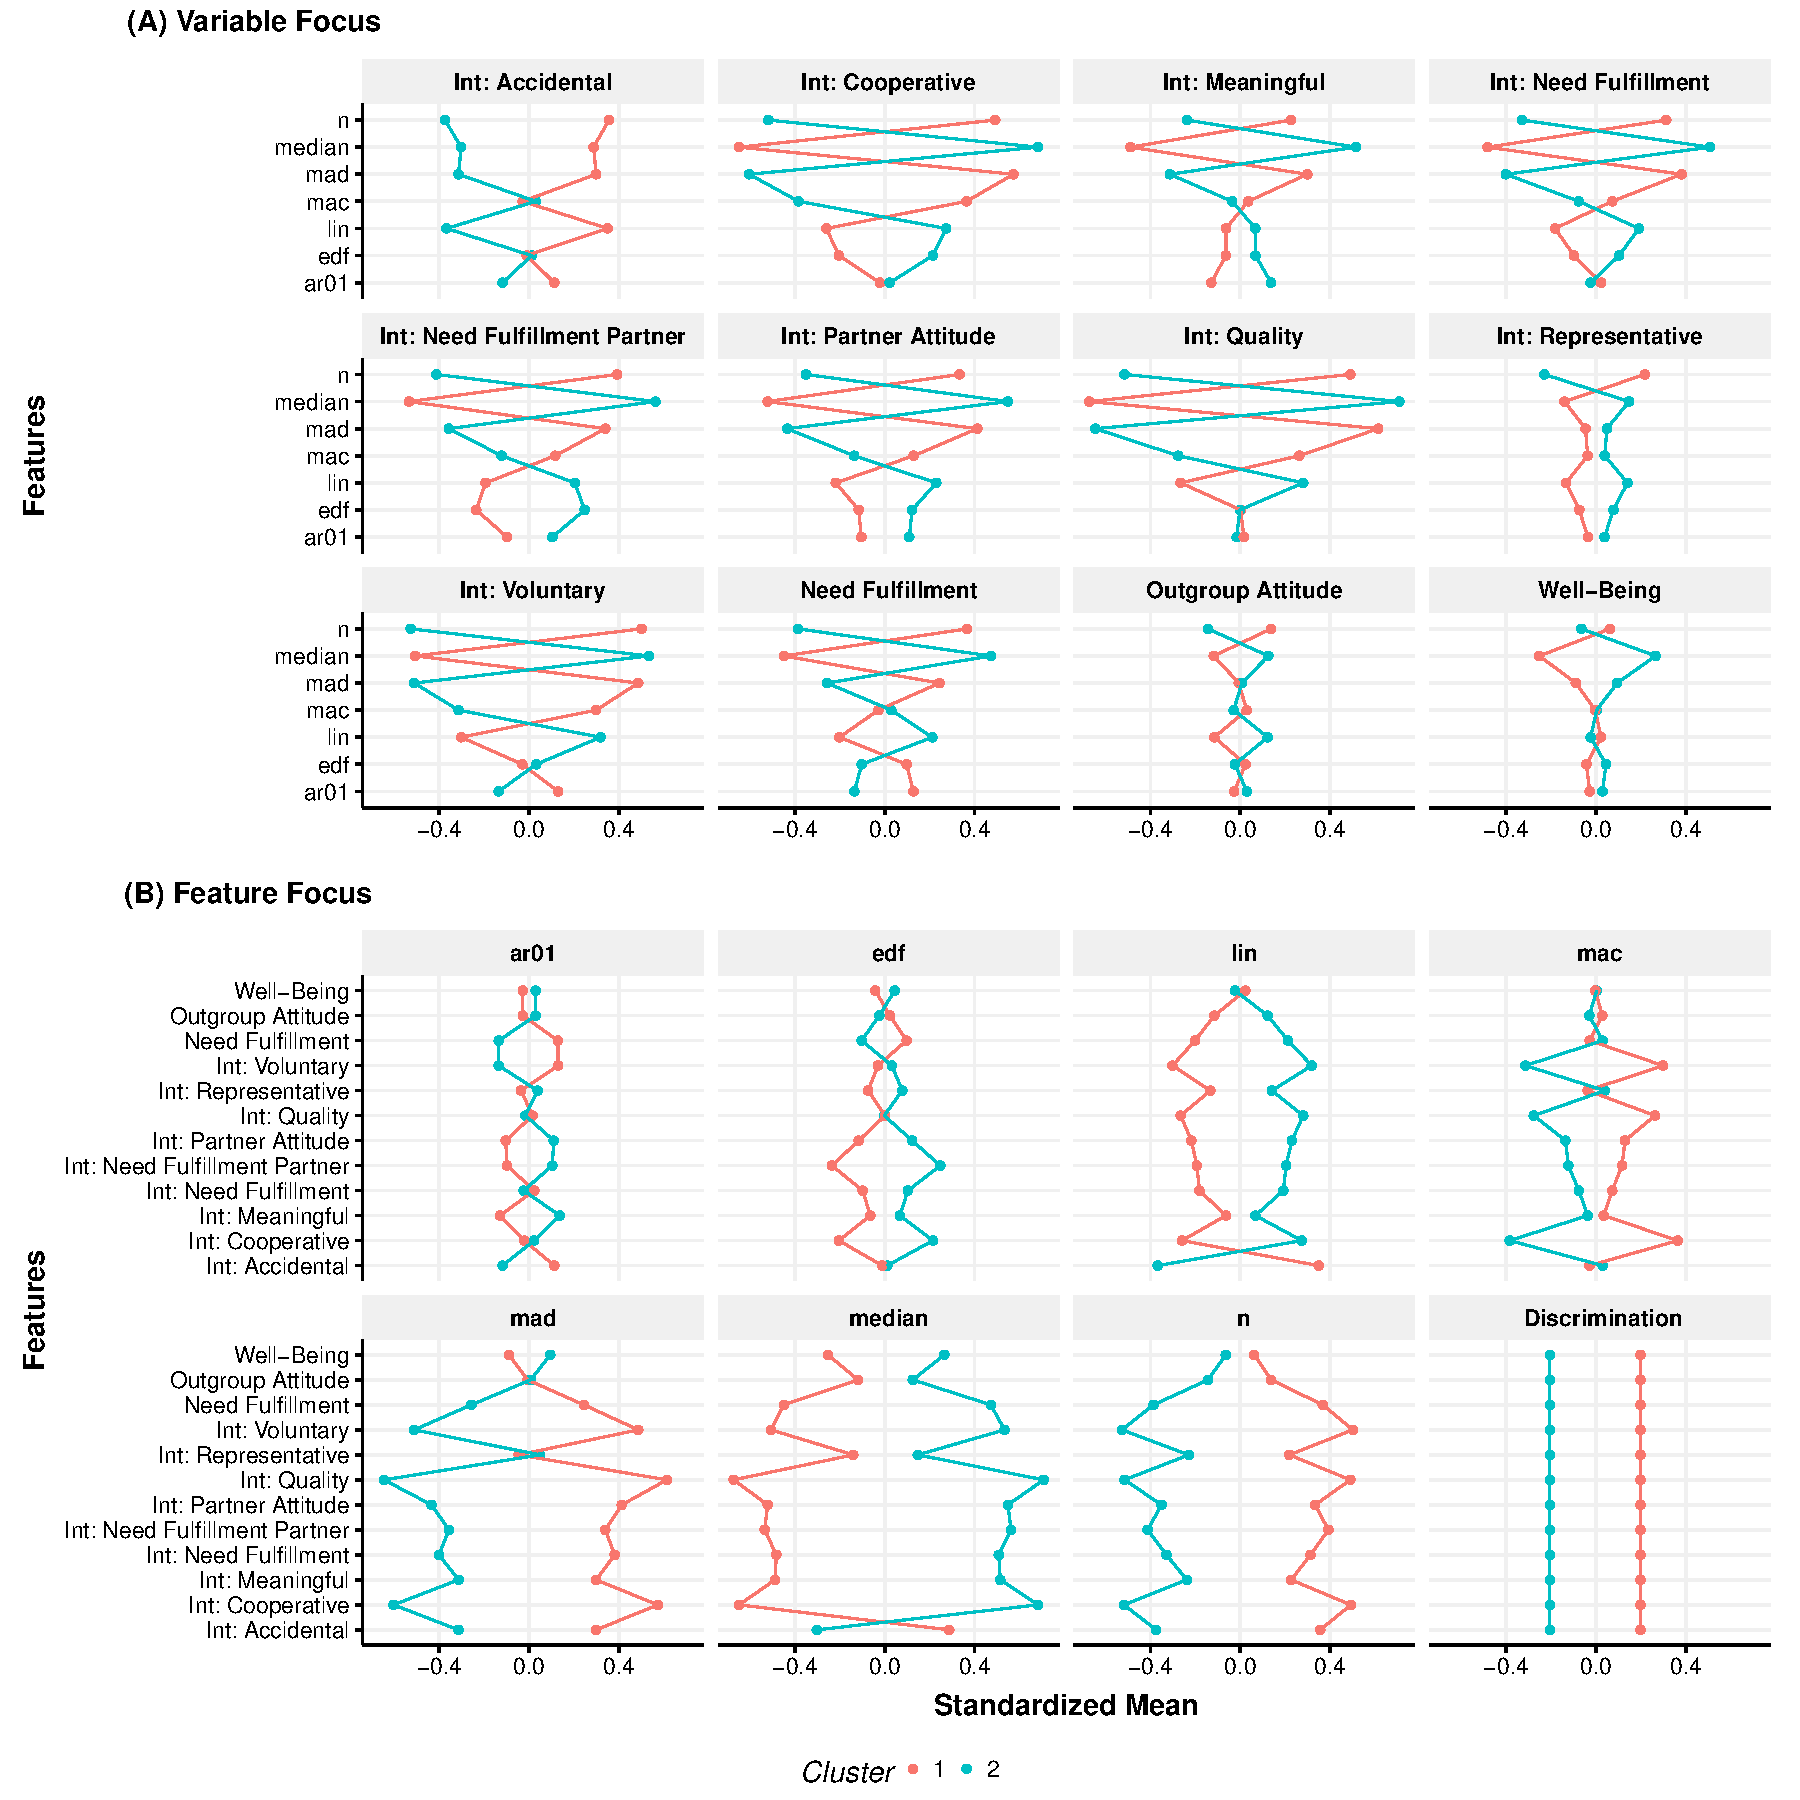
\includegraphics[width=\textwidth]{figures/clusterFeatVarComb.pdf}
  \caption*{Note: \\
  Within the "(B) Feature Focus" subplot, the 'n' and 'Discrimination' comparison variables were not part of the original time series clustering.}
\end{figure}

In the second step, we look at prototypical trajectories of the
clusters. For k-means clustering it is often recommended to use the
average over time of the responses within the cluster
\citep[see \fgrref{fig:clusterTs}][]{niennattrakul2007}\footnote{It is important to note, however, that direct comparability can be a concern, and often times some subset selection or nonlinear alignment is necessary \citep[e.g.,][]{gupta1996}. Additionally, finding cluster prototypes is often substantially easier with embedded clustering methods because in many cases a cluster-level model is estimated as part of the expectation–maximization procedure \citep[e.g.,][]{denteuling2021} or S-GIMME \citep[e.g.][]{lane2019}. For medoid-based clustering algorithms, a common approach is simply using cluster medoid as the prototype \citep{kaufman1990}.}.
Immediately striking are the mean differences, where participants in the
second cluster had more meaningful and fulfilling outgroup interactions
also consistently reported more voluntary and cooperative interactions
but less accidental and involuntary interactions. The same cluster also
reported an increase in need fulfilling interaction over the 30 day
period and an increase in interactions that were representative of the
outgroup. Whereas the other cluster showed a decrease in voluntary,
cooperative, and positive interactions over the 30 days. This
`deterioration' cluster also saw a decrease in general need fulfillment
and experienced well-being over the 30 days (see
\fgrref[B]{fig:clusterTs}). We also see that while interaction
representativeness, outgroup attitudes, well-being are relatively stable
for both clusters, the deteriorating cluster also showed substantially
higher variablity and instability over time (also see
\fgrref[A]{fig:clusterTs}).

Finally, we can also assess the clusters across other person-level
variable \citep[e.g.,][]{monden2022}. This out-of-feature comparison
allows us to check for data artifacts, as well as check whether the
developmental clusters are associated with important social markers and
individual differences. To illustrate artifact checks, we added the
number of measurements into the comparison and find that the
participants in the detereoration cluster on average completed more ESM
surveys and reported on more intergroup interactions than the cluster
with the more positive interactions (see \fgrref[B]{fig:clusterTs}).
While this difference could indicate that the clusters might not
entirely be comparable in the response patterns, we can find some relief
in our data exclusion procedures during which we ensured that the
general time frame and completion rates were not too dissimilar. To
illustrate the utility of individual differences, we compare the two
samples in terms of the participants' self-reported discrimination
experiences in the Netherlands (measured during the post-measurement).
\fgrref[B]{fig:clusterFeatVar} illustrates that participants in the
deteriorating cluster reported substantially higher levels of everyday
discrimination. Thus, both intensive longitudinal and cross-sectional
variables that were not included in the original clustering step can be
used to explore and understand the cluster differences in more detail.

\begin{figure}[!ht] %hbtp
  \caption{Cluster Group Comparisons over time}
  \label{fig:clusterTs}
  \centering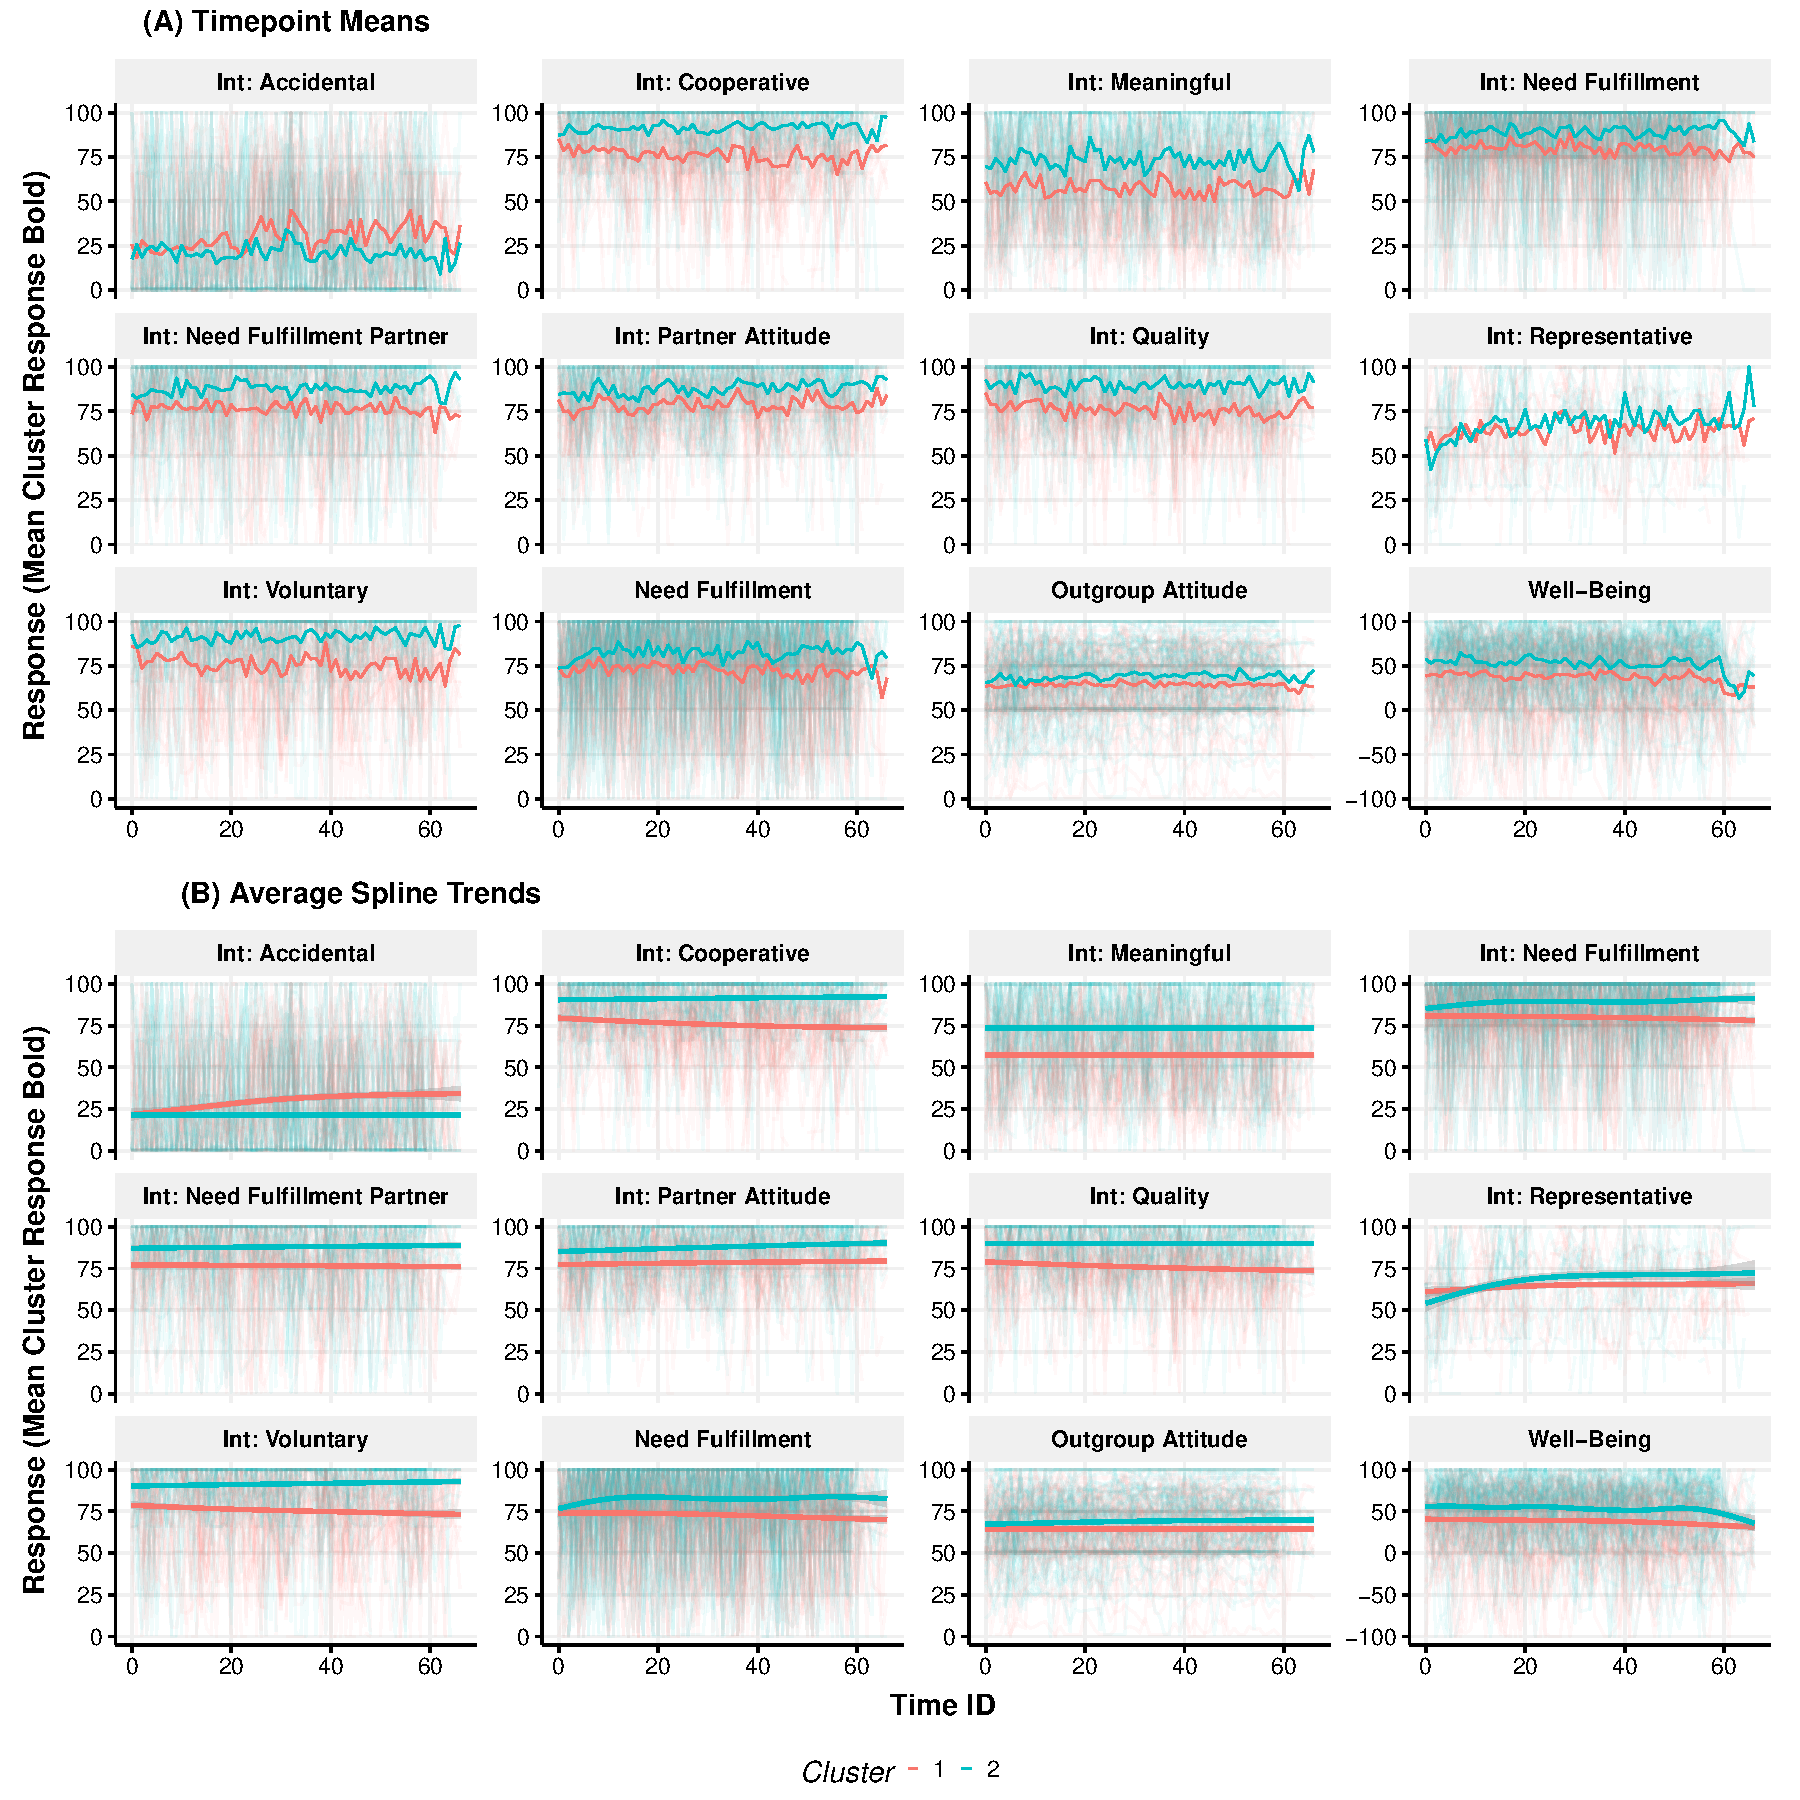
\includegraphics[width=\textwidth]{figures/clusterTsComb.pdf}
  \caption*{Note: \\
  Subplot (A) displays the variable cluster means at every measurement occasion. Subplot (B) shows the GAM spline for each cluster across the measurement occasions.}
\end{figure}


Before we move to the final discussion and conclusions, we would like to comment on the reporting of feature-based time series clustering. Clustering is inherently an exploratory analysis and, as such, each of the analysis steps involves a set of decisions by the user. While this is common for other types of analyses as well, it remains imperative to report the analysis in the most transparent and reproducible manner possible. In our own description of the method, we have separated both the time series features as well as the analysis steps into distinct taxonomies in order to facilitate the transparency of the individual steps and decision moments. Beyond the structures proposed here, \citet{vandeschoot2017} have proposed an extensive checklist for latent trajectory studies. Most of their recommendations and reporting guidelines apply to feature-based clustering as well and might even offer a template for researchers hoping to pre-register their analysis procedures.

\section{Discussion}

NOTES:
The clustering of model parameters is, thus, technically a restrictive sub-form of feature-based clustering --- where lagged regression coefficients, for example, can be considered to be one type of feature capturing a time series. However, beyond model parameters, time series might also be described with any other statistical feature \citep{tiano2021}. 

---

% aims re-iterated
We sought to introduce a flexible and transparent analysis that aids researchers in describing, exploring, and understanding psychological time series data. Such an analysis needs to address the demands of the growing variety of ESM research. In particular, modern describe- and explore analyses should be able to deal with high dimensionality, structural missingness, and diverse time-varying developments. We have argued that feature-based time series clustering is one option that meets this challenge. 

We have methodologically deconstructed the feature extraction, feature reduction, and feature clustering steps and offered methodological as well as conceptual examples for each step. Within this step-wise approach, our article shows that feature-based clustering offers an excellent fit for psychological research practice as both the features as well as the analysis steps are well-established within the field and statistical packages are readily available. Time series features (such as means or linear trends) are not only easy to extract but also hold conceptual meaning for psychological data and can be chosen to address specific research questions (also see \tblref{tab:esmFeatures}). 

\begin{figure}[!hbtp] %hbtp
  \caption{Time Series Clustering Taxonomy}
  \label{fig:tsClustTax}
  \centering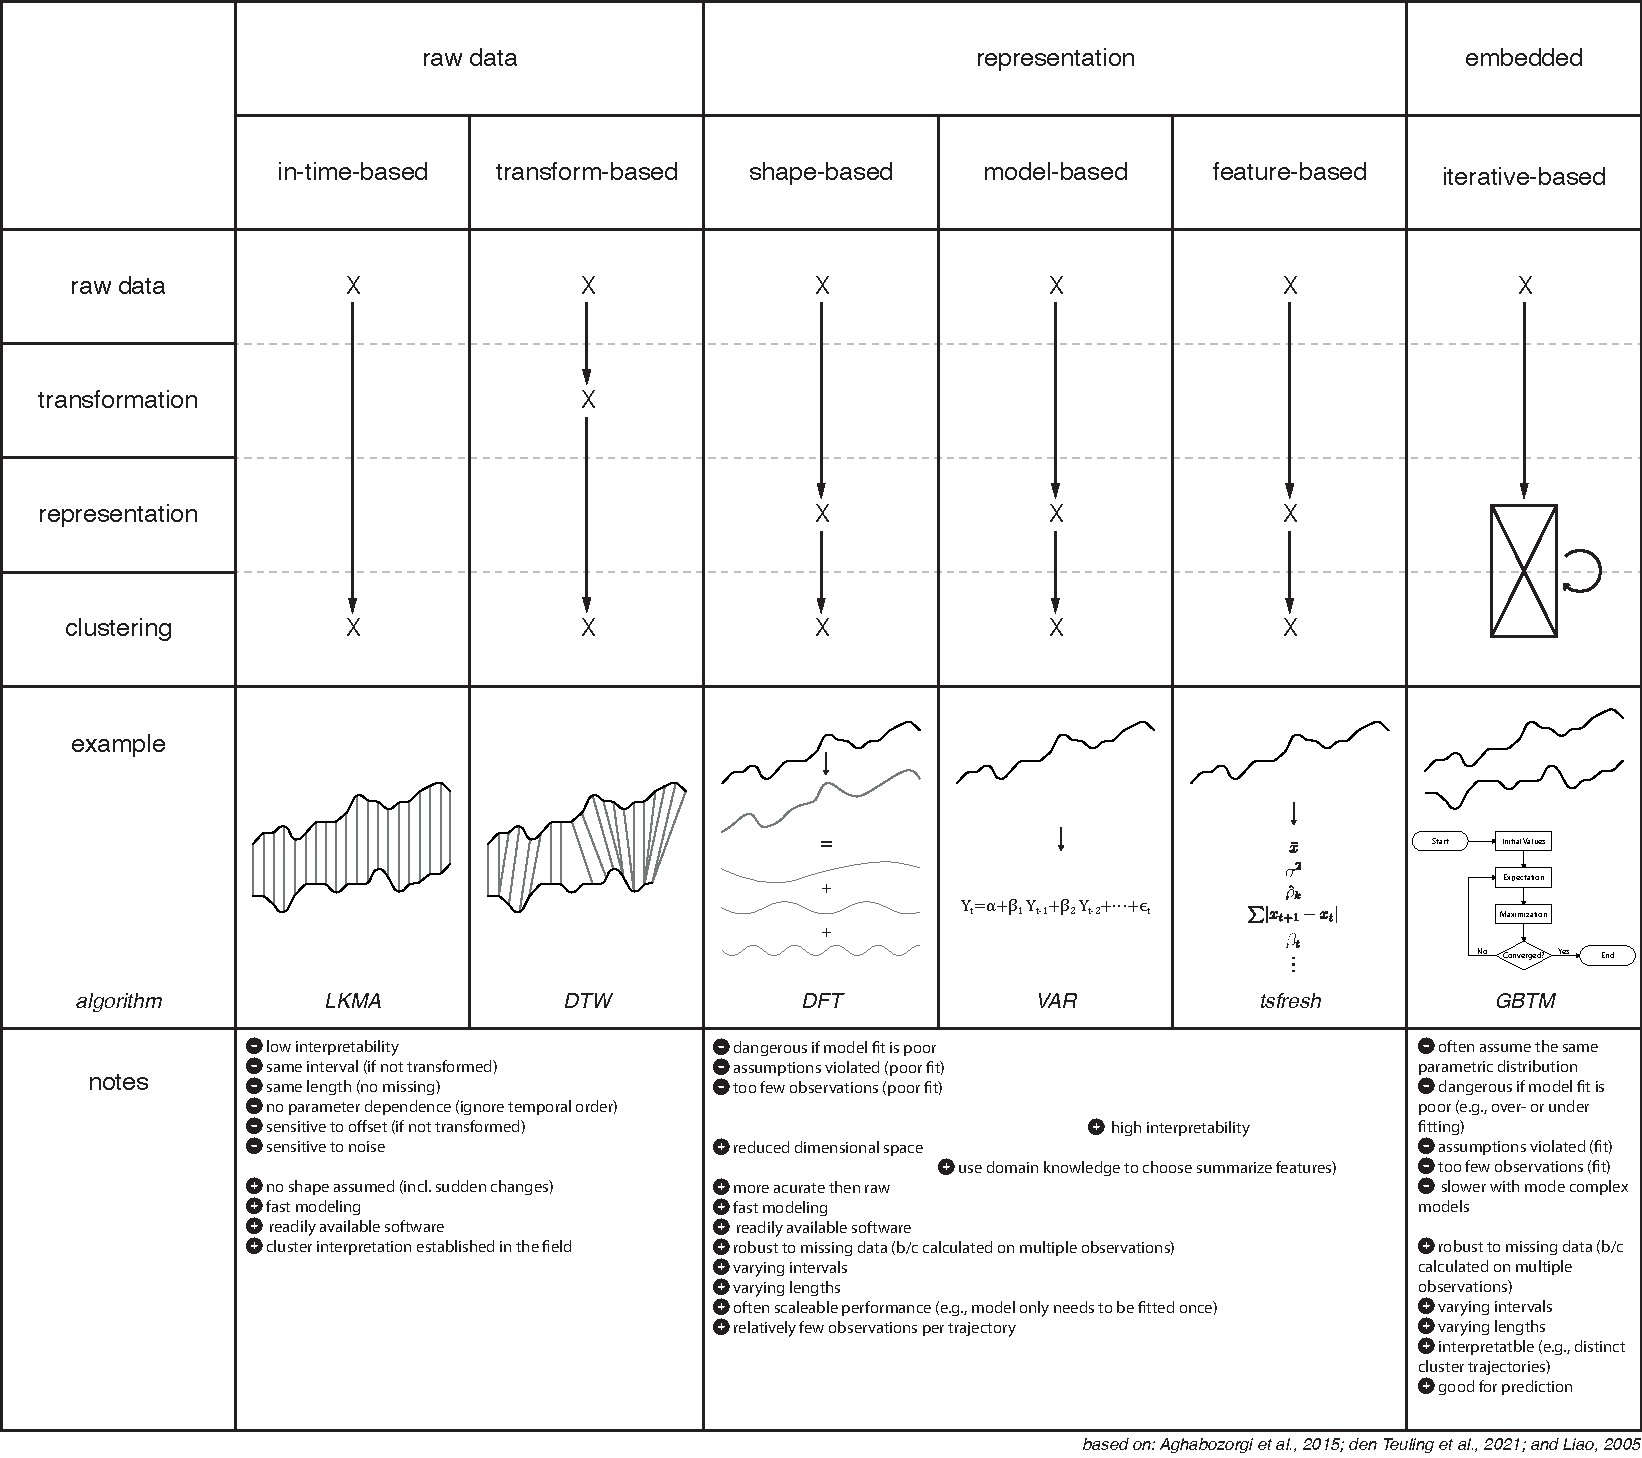
\includegraphics[width=\textwidth]{figures/TS Cluster Flow/tsClustTax.pdf}
  \caption*{Note: \\
  The taxonomy only exemplifies some of the basic differences between a number of common time series clustering approaches. As such, the taxonomy and the notes are neither exhaustive nor complete in distinguishing different approaches. Additionally, terms and labels are used inconsistently across different types of literature and are chosen to avoid overlapping labels.}
\end{figure}

To illustrate the practical utility of the approach, we applied the method to real-life empirical data with diverse conceptualizations, missingness, and nonlinear trends. We make available the full code, custom functions, and illustrations to aid the approachability of the method. In the interpretation step, we also show how the clusters can be compared across the original feature set as well as other meaningful situational and person-specific differences (e.g., see \fgrref{fig:clusterFeatVar}). We also find that for our example of migration experiences, the method was useful in discerning adaptive from more stressful experiences and helped to contextualize the diverging experiences.

As with any statistical method, feature-based time series clustering is not without limitations. 
In particular, feature-based clustering has both a usability as well as robustness limitation in its multiple steps. In terms of convenience, each of the three steps requires users to make an informed decision about the choice of method and algorithm. These additional steps of decision-making and transparency heighten the initial barrier to entry. We hope that our empirical illustration offers a relatively generalizable procedure that showcases the ease of use but clustering unfortunately does not offer a universal one-size-fits-all solution. 

In terms of methodological robustness, the variety of methods in each of the steps also brings with it the potential incomparable results across methods. While the variety and diversity of methods are helpful in finding options even for more complex types of data, different algorithms often offer different results. And even when patterns produce robust clustering solutions across algorithms, individual methods might still have their idiosyncratic shortcomings and might, for example, be sensitive to outliers. 

Notwithstanding the limitations, we believe that feature-based clustering offers an exciting new potential for psychological time series. Across a variety of scientific fields, feature-based time series clustering has been valued for its structuring and simplifying utilities. Within the growing field of psychological time series, modern ESM data is becoming increasingly more complex in terms of participants, variables, and time points. Feature-based time series clusters can aid in reducing these complexities to important and meaningful patterns, an increasingly important task for researchers and practitioners. 



% Tables
% Example
%\input{Tables/descrFullWide}


% Figures


\printbibliography

\appendix

\section{ESM Data Challenges and Promises}
\label{app:ChallengesAppendix}

\subsection{Promises}

Time series clustering has a number of conceptual use cases with psychological data. Prime among them is the ability to reduce the time, variable, and person complexity by extracting and organizing participant-level structures. These reduction and structuring qualities can be essential in detecting phenomena and extracting more abstract functional principles \citep[][]{eronen2021a}. These phenomena and principles can be meaningful differences that distinguish participants in different clusters, as well important patterns, trends, and relationships that participants share within a cluster \citep[e.g.,][]{schrodt2000}. Once distinct groups and patterns have been identified, researchers can examine the extent to which these within-group and between-group structures are associated with other variables of interest, such as personality traits, demographic characteristics, or other psychological constructs \citep[e.g.,][]{monden2022}. By detecting meaningful and robust structures and patterns, time series clustering can, thus, be used to inform the development of robust theories as well as targeted interventions and therapies for individuals, for example, with mood disorders and other psychological conditions \citep[e.g.,][]{borsboom2021, eronen2020}.

However, while clustering can be incredibly useful, arriving at these clusters critically depends on two core challenges. First, time series need to be made comparable in order to identify key (dis)similarities and second, comparable (dis)similarities need to be accurately distinguishing into different groups \citep[e.g.,][]{Aghabozorgi2015}. In practice, most psychological time series cannot be compared based on the raw data itself. This is the case because in most cases the raw time series include too many data points --- sometimes referred to as the dimensionality curse \citep[e.g.,][]{altman2018} --- and, more importantly, individual time points are oftentimes not directly comparable between participants in psychological data and would lead to misspecifications \citep[e.g., ][]{faloutsos1994}. While such issues can be avoided with transformations for highly regular, controlled, and comparable time series such as EEG data \citep[e.g.,][]{huang1985}, most ESM researchers are usually not interested in directly comparing individual timepoints between participants but are interested in developmental patterns and relationships. 

As a result, most psychological time series are summarized via a numerical representation and these numerical summaries are then comparable and used to cluster participants (e.g., \citealp[]{timmerman2013}; see \fgrref{fig:tsClustTax}). Ideally, the representations that summarize the original time series data should (1) capture the original data accurately without loosing too much information, and (2) should be conceptually meaningful \citep[][]{vandermaaten2009}. Extracting accurate and meaningful representations of the time series can be essential for understanding what goes into the clustering algorithm (i.e., assists with explainability) and can be crucial in making sense of the final cluster output \citep[i.e., assists with interpretability; e.g.,][]{Kennedy2021}. 

\subsection{Challenges}

We will briefly consider which challenges modern ESM data introduce and what qualities are called for in an extension of the clustering repertoire. We particularly highlight issues of dimensionality, non-equidistant or missing measurements, an interest in non-stationary trends, as well as inconsistent/diverse time scales. 

Concerning dimensionality issues, especially more abstract psychological experiences often need a wider variety of measurements to be captured adequately. Today, few clinical conditions are captured with a single symptom measure \citep[e.g.,][]{cramer2016}, emotions are rarely assessed in isolation \citep[e.g.,][]{reitsema2022}, and socio-cultural experiences are now widely considered to be multimodal \citep[e.g.,][]{Kreienkamp2022d}. This also means that modern analysis techniques increasingly need be able to accommodate an increased focus on multivariate developments. At the same time, however, an increase in the number of considered variables tends to come at the expense of computational load for model estimations, and clustering models may not converge \citep[the aforementioned dimensionality curse;][]{altman2018}. A modern time series clustering technique should consequently be able to summarize and structure multivariate phenomena without running into computational load issues.

Another common type of data that are measurement regiments that collect data in irregular time intervals (i.e., non-equidistant measurements). Common are, for example, procedures where participants are asked to respond at random times throughout the day (i.e., signal-contingent) or following specific natural events of interest \citep[i.e., event-contingent; see][]{shiffman2008, myin-germeys2018}. Under such conditions data tends to violate the equidistance assumption that is expected by many time series models \citep[][]{hamaker2017}. Smaller issues of non-equidistant data can be avoided with transformations \citep[e.g., dynamic time warping,][]{berndt1994} or newer modeling procedures \citep[e.g., continuous-time models;][]{dehaan-rietdijk2017} but for many analyses, including some cluster approaches, non-equidistant measurements remain a prevalent issue. 

Structural missingness remains an even more strenuous challenge. Structural missingness occurs when data is missing because it logically cannot be collected \citep[as opposed to probabilistically missing data;][]{little2020, mclean2017}. Often, however, researchers might want to include variables in their models that are not available under all conditions. Follow-up and event-contingent questions are a common example in ESM studies. Researchers, for example, ask about the frequency, intensity, or duration of symptoms --- but only if a symptom was present \citep{kivela2022}. Such approaches become specifically critical in cases of sensitive questions such as questions about suicidal ideation or other potentially trauma-inducing questions \citep[e.g.,][]{glenn2022}. The most common practice for structurally missing data is to either exclude the variable or any measurement that has no structurally missing data \citep[e.g.,][]{lavori2008}\footnote{This is the case because the most commonly used models require complete data \citep{schafer2002} and structurally missing data cannot be imputed as it logically does not exist \citep[e.g.,][]{lavori2008}.} --- neither option suits a research question that wishes to include variables with common structural missingness, such as event-specific or follow-up questions. In short, new clustering approaches should be able to deal with structurally missing data in order to address modern ESM data.

When it comes to studying developmental trajectories, psychological researchers are often also interested in nonstationary processes because they are more representative of the complex, dynamic behavior of the human mind. In psychology, nonstationary processes are typically used to study phenomena such as cognitive development \citep[][]{quartz1997}, decision-making \citep[][]{ratcliff2016}, and emotion dynamics \citep[][]{bringmann2018b}. These processes are often characterized by changes in the underlying statistical properties of the data over time, such as changes in the mean or variance \citep[][]{molenaar2009}. Especially when considering changes in mean levels, researchers are often interested in nonlinear changes because they describe human functioning better. For example, in decision making people might switch between choices \citep[][]{ratcliff2016}, or patients reducing medication might experience mood swings \citep[][]{helmich2020a}. Similarly, psychologists are often also interested in how variances change over time. This is especially the case because several changes in an individual's variance have been found to be indicative of critical changes, including depression relapses and symptom shifts more generally \citep[e.g.,][]{schreuder2020, wichers2020}. There is, thus, also a need for time series clustering algorithms that capture nonstationary processes, including nonlinear trends.

Psychological time series often exhibit complex patterns and relationships that can change over different time scales. For example, a time series of daily mood ratings may show a weekly pattern, with higher ratings on the weekends and lower ratings during the week. At the same time, the series may also exhibit a longer-term trend, with overall mood levels increasing or decreasing over the course of several months or years \citep[e.g.,][]{Ram2014}. \sout{These different time scales can be studied separately or in combination, using different statistical techniques and modeling approaches \citep[][]{bertenthal2007, jeronimus2019a}.} Different time scales can become an even more difficult issue when different variables in a model develop on different time scales \citep{bringmann2022b}. Different time scales are thus also a concern clustering approaches should be able to address.

%These shortcomings, however, stand in sharp contrast with the types of data researchers commonly collect and do not align with common research interests in the field. Psychological researchers might, for example, collect data based on the occurrence of natural events, which tends to result in non-equidistant measurements \citep[e.g.,][]{myin-germeys2018, hamaker2017} and context-specific missingness that cannot be imputed, for instance, interaction quality perceptions \citep[e.g.,][]{kivela2022, lavori2008}. At the same time, researchers are often specifically interested in non-stationary developments, looking, for example, at how symptom levels and -variations change over time --- often abruptly and non-linearly \citep[e.g.,][]{bringmann2018b, helmich2020a}.


\section{Background of the Proposed Psychological Time Series Features}
\label{app:FeatureBackground}

With its rich history, a staggering variety of time series features have been proposed, not all of which are meaningful for psychological time series. As an example, \citet{wang2006} propose a set of nine statistical features for describing a trajectory: (1) trend, (2) seasonality, (3) periodicity, (4) skewness, (5) kurtosis, (6) serial correlation, (7) non-linearity, (8) self-similarity, and (9) chaos \citep[also see][]{fulcher2013}. \citet{adya2001} proposed a total of 28 features relevant for forecasting, which largely fit within the selection proposed by \citet{wang2006}. A final illustration comes from a commonly used software package for feature extraction `tsfresh', which allows users to extract a total of 794 features to describe all kinds of aspects of a time series \citep[][]{christ2018}. 

Given that there are hundreds of possible features to describe psychological time series, one approach to choosing relevant features would be to extract a large number of features and then assess which features are most effective at capturing differences in the time series \citep[e.g.,][]{christ2018}. However, such an approach is not always advisable for psychological time series. For one, features should reduce the data dimensionality --- it would thus not necessarily be advisable to describe 60 ESM measurements with 794 time series features. More importantly, however, careful feature extraction can be crucial in the interpretability and explainability of the results. This is particularly the case when features have a conceptual or psychological meaning. Taking the concept of well-being as an example, psychologists might be interested in whether certain participants tend to have higher well-being in general (i.e., mean) or whether some participants fluctuate between extremely high and low well-being (i.e., variance). But psychologists might not necessarily be interested in the exact time point after which 50\% of the summed well-being values lie (i.e., relative mass quantile index) or how much different sine wave patterns within the well-being data correlate with one another (i.e., cross power spectral density). We will, thus, propose and describe a set of time series features that have a strong backing within the ESM literature and as such offer a reasonable starting point for most concepts within the field.



\paragraph{Central Tendency} Central tendency refers to the statistical measures that represent the ``middle" or ``average" of a set of data. The most common measures of central tendency are the mean, median, and mode (Hopkins, 2020). As a familiar statistic from probability theory, the central tendency sits at the heart of many fundamental questions about psychological time series. Researchers might, for example, be interested in whether ``Over a one month period, are some people happier than others?''. A recent review paper pointed out that the relatively simple mean statistic, is often overlooked in psychological time series analyses but is usually essential for understanding psychological differences \citep{bringmann2018c}. As such, several time series modeling approaches now advocate for conscious consideration of the mean \citep[e.g.,][]{bringmann2017a}. As with cross-sectional data, for time series data the appropriate measure of central tendency depends on the specific characteristics of the data being analyzed. For instance, if the data are normally distributed, the mean is often an appropriate measure. If the data are skewed or have outliers, the median may be a better choice \citep{weisberg1992}.

\paragraph{Variability} Variability captures the degree to which a set of data differs from the central tendency and is sometimes also referred to as the dispersion or spread of the data \citep{weisberg1992}. In time series analyses, variability is conceptually important because it provides information about the distribution and diversity of the data. Especially within-person changes in variability have recently received increasing attention because they can be a potent early warning signal in psychological time series \citep{helmich2020a, vandeleemput2014}. A marked within-person increase in variance has, for example, been found to precede crucial transitions --- often considered to be part of a phenonenon know as critical slowing down \citep[i.e., anomalous variances; e.g.,][]{scheffer2009, wichers2019}. 

But also more global person-level differences in time series variability have been found to be crucial and relate to important psychological questions. Person-specific differences in variability have, for example, been found to be indicative of worse psychological states \citep{myin-germeys2018}. And, similarly, person-level differences have also been associated with higher levels of psycho-pathological recurrences among depression patients \citep{timm2017}. As such, psychological researchers and practitioners are often empirically interested in person-level differences in variability. Researchers on polarization and radicalization might for example ask: "Are people settled in their attitudes towards migrants or vary across the measurement period?''

Methodologically, there are several measures of variability, including the range, standard deviation, and variance. The appropriate measure to use depends on the specific characteristics of the data being analyzed. For normally distributed data variances and standard deviation are often preferred, whereas data with outliers or nonparametric distributions are often better described with robust variability measures such as the median absolute deviation \citep{weisberg1992}.

\paragraph{(In)stability} Instability captures the average change between two consecutive measurements \citep{ebner-priemer2009}. While instability is conceptually related to the variability feature, variability does not take into account temporal dependency, whereas instability looks at the `jumpy-ness' of the data over time. In other words, variability reflects the range or diversity of values in a time series data, while instability reflects the fluctuation or inconsistency in a time series data over time  \citep{trull2008}. For example, if a person has rapid and extreme changes in mood their mood is highly unstable, while if a person's mood responses span a wide range over the entire study period, their mood is highly variable \citep{jahng2008}. Within psychological time series, instability measurements have especially been important in the research of borderline personality disorder \citep{trull2008} and suicidality \citep{kivela2022}, but also in understanding early warning signals more generally \citep{wichers2019}. Conceptually, the instability feature, thus, relates to a broad range of research questions, including: ``Do changes tend to be slow and gradual or fast and abrupt?" Methodologically, (in)stability measurements often look at the average change between two consecutive measurements, such as the mean absolute change \citep[e.g.,][]{ebner-priemer2009,barandas2020}. 

\paragraph{Self-similarity} Self-similarity in time series data refers to the property of a time series to exhibit similar patterns of behavior over different time scales \citep{dmello2021}. That is, self-similarity describes how much a measurement carries over to future measurements. There are two main ways in which experiences tend to be connected to future experiences in psychological time series --- resistance to change and seasonality. Both forms of self-similarity relate to different types of research questions. 

Resistance to change is the self-similarity of a measurement with its next measurement and is often referred to as inertia \citep{kuppens2010}. If inertia is high a development tends to stay in a certain state or continues to move towards a certain direction. Because high inertia is resistant to change, in emotion dynamics high inertia has been found to be indicative of underreactive systems and to be characteristic of psychological maladjustment \citep{kuppens2010}. In a similar vein, high inertia at baseline was even predictive of the initial onset of depression \citep{kuppens2012}. Conceptually, inertia is more broadly connected to research questions such as: ``Do patients stay in a depressed mood for several measurements?'' One way to measure inertia in time series data is through the use of autocorrelations or autoregressions with a lag-1, which look at the correlation between a given time series and itself at the previous measurement occasion. High autocorrelation values can indicate high levels of inertia, while low autocorrelation values may indicate a more unpredictable or volatile time series \citep{dejonckheere2019}.

Seasonality is the self-similarity of a measurement that returns in a cyclical manner and is often also referred to as periodicity \citep{gregson1983}. Periodicity in psychological time series data, thus, refers to the presence of recurring patterns at regular intervals. In psychological time series, these cyclical patterns are not only dangerous for models that assume stationarity \citep{beal2015} but can be interesting psychological properties in their own regard \citep{epskamp2018, schmittmann2013}. Humans generally live in seasonal environments, including, for example, exam periods at universities \citep{fuller2003}. But also more internally, personality manifestations, for example, have long been assumed to develop cyclically \citep{cattell1957}. The associated research questions can be driven by an understanding of external seasonality factors such as: ``Do participants drink more alcohol on Fridays?'' But research questions can also address periodic patterns as they may be the result of underlying psychological processes: ``Does stress increase with fatigue cycles?'' Similar to inertia, periodicity is often measured using autocorrelations but then with the lag of the seasonality or cycle (e.g., daily, seven days, one month, one semester). Periodicity can additionally be captured using spectral analysis or decomposition, such as with wave patterns \citep[e.g., fourier or wavelet transformation; e.g.,][]{mayor2022}.

\paragraph{Linear Trend} Linear trends in time series data refer to the presence of a straight-line development of a variable being measured. This type of trend can be observed when there is a consistent increase or decrease in the data over time \citep{nyblom1986}. For psychological time series, researchers have, for example, pointed out linear trends in interpersonal communications \citep{vasileiadou2014}, and emotion dynamics \citep{oravecz2016}. Linear trends are often the simplest way of assessing whether a psychological theory of change is appropriate \citep{gottman1969}. In empirical practice, linear trends are, thus, a common research interest for psychological time series data. ``Do patient symptoms improve consistently?'' or ``Does worker productivity decline continuously?'', are familiar types of research questions. Mathematically, such linear trends are commonly captured using (piecewise) linear regression coefficients, but also using differential equations \citep{chow2019}. 

\paragraph{Nonlinearity} Changes in psychology are not always linear, instead nonlinearity is a common feature of psychological time series \citep{hayes2007}. As an example, episodic disorders, such as depression, are most likely best described as non-linear systems \citep{hosenfeld2015}. Similarly, patients in recovery from depression showed sudden changes in the improvement of depression \citep{helmich2020a}. But also substance abuse \citep{boker1998} or attitude changes rarely develop linearly \citep{vandermaas2003}. For psychological researchers, nonlinear developments are, thus, important in two regards. Firstly, nonlinearity as a deviation from linear trends is an important feature defining many psychological time series and secondly, the shape and structure of the nonlinear trend can be essential in understanding the important changes and transitions of human experiences \citep{chow2019}. Conceptually, researchers might accordingly have research question about the type of the development: ``Is the development of anxiety a nonlinear process?'' as well as the shape and structure of the development: ``Does anxiety change as a sudden or smooth transition?'' Accordingly, researchers can capture the type of development with nonlinearity parameters such as the bicoherence metrics \citep{cuddy2009}. The structure of nonlinear trends is often mathematically more difficult to capture \citep{castro-alvarez2022a}. Common ways to capture the trends include the use of polynomial- and differential equation parameters or more broadly to capture how `wiggly' the trend line is (e.g., estimated degrees of freedom of GAM spline models; similar to the number of spikes \citealp[]{caro-martin2018}). 

\end{document}
